\documentclass[11pt,twoside]{extarticle}
\usepackage{floatrow}
\usepackage{etex}
\usepackage[english]{babel}
\usepackage{url}
\def\UrlBreaks{\do\/\do-}
\usepackage[breaklinks]{hyperref}
\usepackage{comment}

\usepackage[figuresright]{rotating}
\usepackage[margin=1.2in]{geometry}
\usepackage{setspace}
\renewcommand{\baselinestretch}{1.3}
\usepackage{booktabs, multicol}
\usepackage{threeparttable}
\usepackage{pdflscape}
\usepackage{xcolor}
\usepackage{amstext}
\usepackage{pgfplots}
\usepackage{color}
\usepackage{soul}
\usetikzlibrary{shapes,positioning,matrix,calc,shapes,shapes.multipart,shapes.misc,arrows,chains,fit,plotmarks}
\usetikzlibrary{decorations.text}

\usepackage{eurosym}
\usepackage{amssymb}
\usepackage{amsfonts}
\usepackage{afterpage}
\usepackage{epsfig}
\usepackage{upgreek}
\usepackage{commath}
\usepackage{enumitem}
\usepackage{subfigure}
\usepackage{indentfirst}
\usepackage{xr}
\usepackage{dsfont}
\usepackage{cleveref}
\usepackage{titlesec}
\usepackage{titling}
\usepackage{multibib}
\usepackage{makecell}
\usepackage{soul}
\usepackage{arydshln}
\usepackage{mathrsfs}
\usepackage{ragged2e}
\newcites{online}{References}
\allowdisplaybreaks

\usepackage[normalem]{ulem}

\setcounter{MaxMatrixCols}{10}

\newtheorem{theorem}{Theorem}
\newtheorem{acknowledgement}{Acknowledgement}
\newtheorem{algorithm}{Algorithm}
\newtheorem{assumption}{Assumption}
\newtheorem{axiom}{Axiom}
\newtheorem{case}{Case}
\newtheorem{claim}{Claim}
\newtheorem{conclusion}{Conclusion}
\newtheorem{condition}{Condition}
\newtheorem{conjecture}{Conjecture}
\newtheorem{corollary}{Corollary}
\newtheorem{criterion}{Criterion}
\newtheorem{definition}{Definition}
\newtheorem{example}{Example}
\newtheorem{observation}{Observation}
\newtheorem{exercise}{Exercise}
\newtheorem{fact}{Fact}
\newtheorem{lemma}{Lemma}
\newtheorem{notation}{Notation}
\newtheorem{problem}{Problem}
\newtheorem{proposition}{Proposition}
\newtheorem{remark}{Remark}
\newtheorem{solution}{Solution}
\newtheorem{summary}{Summary}
\providecommand*{\theoremautorefname}{Theorem}
\providecommand*{\factautorefname}{Fact}
\providecommand*{\lemmaautorefname}{Lemma}
\providecommand*{\propositionautorefname}{Proposition}
\providecommand*{\corollaryautorefname}{Corollary}
\providecommand*{\definitionautorefname}{Definition}
\providecommand*{\remarkautorefname}{Remark}
\providecommand*{\subfigureautorefname}{Subfigure}
\providecommand*{\algorithmautorefname}{Algorithm}
\providecommand*{\assumptionautorefname}{Assumption}
\newenvironment{proof}[1][Proof]{\noindent \textbf{#1.} }{\ \rule{0.5em}{0.5em}}
\geometry{left=1.2in,right=1.2in,top=1.3in,bottom=1.3in}
\renewcommand{\baselinestretch}{1.3}
\newcommand{\newln}{\\&\quad\quad{}}
\newcommand{\parenthnewln}{\right.\\&\left.\quad\quad{}}
\usepackage{bbm}

\usepackage{longtable}
\usepackage[para]{threeparttablex}

\usepackage{float}
\usepackage[titletoc,title]{appendix}
\raggedbottom

\usepackage{amsmath}
\usepackage{bm}
\usepackage{lineno}

\usepackage[T1]{fontenc}
\usepackage{palatino}

\usepackage{graphicx}

\hypersetup{
   colorlinks=true,linkcolor=blue,citecolor=blue, filecolor=magenta, citebordercolor=yellow,
   linkbordercolor = magenta
}

\usepackage{graphicx}
\graphicspath{{../output/figures/}}
\usepackage{subfigure}
\floatsetup[figure]{font=footnotesize}

\floatsetup[table]{capposition=top}
\floatsetup[table]{font=footnotesize}

\floatsetup{style=plain,footposition=bottom}
\floatsetup[figure]{capposition=bottom}

\usepackage{multirow}
\newcommand{\specialcell}[2][c]{%
        \begin{tabular}[#1]{@{}c@{}}#2\end{tabular}}

\makeatletter
\renewcommand\@makefntext[1]{%
    \parindent 1em%
    \@thefnmark.~#1$\qquad$}
\makeatother

\usepackage{tabularx}
\newcolumntype{R}{>{\raggedleft\arraybackslash}X}
\newcolumntype{L}{>{\raggedright\arraybackslash}X}
\newcolumntype{C}{>{\centering\arraybackslash}X}

\usepackage[figuresright]{rotating}

\usepackage[font=normalsize,format=plain,labelfont=bf,up,textfont=up,justification=centering]{caption}
\captionsetup[table]{labelsep=space}
\captionsetup[figure]{labelsep=space}
\addto\captionsenglish{%
\renewcommand{\figurename}{FIGURE}
\renewcommand{\tablename}{TABLE}}
\renewcommand{\thesubfigure}{(\Alph{subfigure})}

\usepackage{natbib}
\newcommand{\cites}[1]{\citeauthor{#1}'s (\citeyear{#1})}

\usepackage{pdflscape}

\usepackage[titletoc]{appendix}
\usepackage{titletoc}

\title{Manufacturing Enemies in Political Contests}
\author{Haotian (George) Bai\thanks{I thank conference and seminar participants at Oxford. I extend special thanks to Prof.\ Jean-Paul Carvalho (Oxford).}}
\date{\today}

\begin{document}

\maketitle

\begin{abstract}
Why do political groups enact identity-coded policies (symbolic policies) against domestic minorities? 
I study a two-sided security contest with within-group collective action into a probabilistic-voting model with retrospective accountability. Symbolic policy lets a security-advantaged \emph{hawkish} party manufacture a visible threat that relaxes majority free-riding, makes its coercive-capacity advantage electorally salient, and substitutes identity politics for economic competence. A two-period model shows the hawk's vote share is non-monotonic in the grievance it manufactures. Once the hawk generate sufficient minority mobilisation, future conflict continues despite incumbent policies. 
I further study the long-run equilibria under symbolic policy-making. Iterating the same myopic-retrospective swing rule under an salience shocks embeds the system in a perturbed Markov chain whose long-run regime (a self-sustaining hawk trap or recurrent Haw-Dove cycles) is selected by the depreciation rate of minority mobilisation. 
India's cattle-slaughter legislation and other cases are consistent with each prediction. I discuss why banning symbolic policies may backfire.\\

\emph{JEL Codes: D72, D74, P16, Z18}.

\end{abstract}
\clearpage

\begin{quote}
\textit{``Only one thing is worse than communal war --- and that is when your government exploits communal differences, stokes ethnic and religious fears, all in the pursuit of power.''}

\hfill --- A. Sivanandan, \textit{``Ethnic Cleansing in Sri Lanka''}
\end{quote}

\section{Introduction}

% Paragraph 1 — Opening: the phenomenon

There has been a widespread rise in identity-coded policies (symbolic policies) targeting domestic minority groups in electoral democracies. By symbolic policies, I mean deliberate control over cultural, religious, and ethnic identities on minority groups. These policies include restrictions on diet, dress, marriage, or language regulations, chosen by an elected majority party and directed at a visible domestic out-group. In the last decade, legislative waves in major Indian states have criminalised cow-slaughtering with penalties of up to ten years' imprisonment.\footnote{The cumulative state-by-state rollout of all six ban types is shown in \autoref{fig:policy_cumulative_rollout}, with the year-by-year coverage tabulated in Appendix~\autoref{tab:policy_timing}. Following \citet*{dasguptaNutritionalCostBeef2023}, I tracked policy-enactment dates across state legislative records.} Between 2012-2018, over forty cow-related deaths were documented, whose victims were mostly Muslim.\footnote{\href{https://www.hrw.org/report/2019/02/19/violent-cow-protection-india/vigilante-groups-attack-minorities}{Human Rights Watch (2019), last access Apr 17\textsuperscript{th}, 2026}.} The pattern has been repeated across electoral democracies, from the post-2016 anti-immigration turn in the United States, to the Uribista policies under Álvaro Uribe Vélez. Such polices are also seen in non-democracies with political competition.\footnote{Iranian principalists deploy hijab enforcement and morality-policing campaigns to combat economics reformists when they gain popularity \citep*{bajoghliIranReframedAnxieties2020}. Chinese Communist Party (CCP) has divergent policies on ethnic groups as Politburo faction shifts \citep*{leiboldEthnicPolicyChina2013}. \citet*{francoisFactionsNondemocraciesTheory2023} introduces CCP factions, policies, and welfare in China. \citet*{francoisHowPowerShared2015} documents ethnic-political contests in Africa.} These features also defy economic theories of political accountability in political contests \citep*{barroControlPoliticiansEconomic1973,ferejohnIncumbentPerformanceElectoral1986}. Why does a rising number of political groups obtain and sustain power through a non-pivotal minority group?

% Paragraph 2 — Consequently: policy and scholarly interest, and the gap

Consequently, using domestic minorities as a political tool has become the centre of debate on the democratic process and economic development. In 2019, India's Citizenship Amendment Act ignited the largest sustained urban protest since independence \citep{jaffrelotModisIndiaHindu2021}.\footnote{The \emph{Woman, Life, Freedom} protests in Iran after the 2022 death of Mahsa Amini and the wide-spread anti-immigrants Republican campaigns before the 2024 United States presidential election show similar patterns.} However, political economists have not fully understood why majority parties choose such policies in the first place, why voters reward them, and why the same mechanism produces durable one-party dominance in some polities and recurrent turnovers in others.

% Paragraph 3 — Placing the paper, stating the aim, and the toolkit

This article introduces the manufacturing of enemies in political contests to the economics of identity and electoral competition \citep*{shayoModelSocialIdentity2009,glaeserPoliticalEconomyHatred2005,gennaioliIdentityPolitics2023}.\footnote{A large literature has captured electoral mobilisation of communal violence by majority parties in divided democracies.} My aim is to explain why elected majority parties choose symbolic policies against domestic minorities, and to characterise the long-run consequences of doing so for political competition and social conflict. In attempting to do so, I draw on developments in contest theory and the political economy of electoral accountability.

% Paragraph 4 — The model

In my model, symbolic policy activates a two-sided contest over public security (in identity) between a majority group and a domestic minority. Following \citet*{baligaStrategyManipulatingConflict2012}, two parties compete for the majority's vote: one with a comparative advantage in delivering economic public goods, the other in coercive and organisational capacity. The minority is composed of agents sensitive to their minority identities (e.g.\ Muslim groups in India). They mobilise to preserve their identity from the majority's encroachment (through protest or violence). Subject to the collective-action problem, mobilisation only occurs when grievance among their members is large enough. The majority base faces the symmetric problem. The greater the intensity of symbolic policy, the larger the grievance the minority's mobilisation averts, and the more the majority's free-riding is relaxed by the visible threat its own counter-mobilisation creates. The electoral return to symbolic policy is therefore highest when the security-oriented party (\emph{Hawk}) has an organisational advantage that is unobserved in peaceful conditions, or when the economic potential of its opponent (\emph{Dove}) is sufficiently large that it cannot be offset on the consumption dimension alone.

% Paragraph 5 — Linking the model to observed patterns

This enables me to link the manufacturing of enemies to the economic and political transformations that have accompanied recent electoral democracies. The most important changes were the rise of redistributive politics after the Cold War, the widening of the electoral franchise through liberalising the minority in post-colonial areas, and the emergence of parties whose organisational base lies in religious, paramilitary, or coercive associations. I show that manufacturing enemies, by making the security dimension of contest electorally salient, comes at the cost of real economic and social disruption. I aim to develop a unified framework for understanding the contemporary use of symbolic policy in otherwise disparate settings: India's cow-slaughter bans under the BJP \citep{jaffrelotModisIndiaHindu2021}, the Republican Party's post-2016 pivot to immigration and domestic-security framing in the United States \citep{sidesIdentityCrisis20162019,mutzStatusThreatNot2018}, the persistence of morality-police enforcement in Iran \citep{bajoghliIranReframedAnxieties2020}, and the consolidation of Uribismo in Colombia \citep*{acemogluMonopolyViolenceEvidence2013}. It suggests one possible explanation for the prominent role that security-coded mobilisation plays during periods of economic liberalisation, when the non-hawkish coalition's comparative advantage in economic delivery is at its greatest.

% Paragraph 6 — Model setup and the baseline two-period game

I formalise this mechanism in a two-sided Tullock contest with within-group collective action, embedded in a probabilistic-voting game with retrospective accountability. The polity is partitioned into a Majority, represented in the electoral arena by two parties and a non-voting Minority. The two parties differ along two technological dimensions: the Hawk has higher coercive capacity but lower public-goods capacity. In each period the incumbent commits to a symbolic-policy intensity; conditional on $d$, the Majority and Minority each choose mobilisation effort subject to a private quadratic cost, and the within-period contest produces a closed-form equilibrium dominance probability for each party. The Minority's effective stake decays at $\rho$. The voter is \emph{myopic-retrospective}: she observes the realised state, computes each candidate's stationary per-period welfare under his best-reply at that state, and votes for whoever delivers more by weighting the Hawk's security advantage against the Dove's economic advantage and the real economic destruction symbolic policy imposes. My baseline analysis sloves a two-period game with. The period-1 Hawk anticipates how its period-1 policy shapes the inherited mobilisation that the period-2 voter then evaluates against the period-2 incumbent's stationary best-reply. I discuss assumptions in \autoref{sec:model_v3}.

% Paragraph 7 — Long-run extension

To study the long-run consequences of manufactured enemies, I iterate the same within-cycle game under the same myopic-retrospective voting rule, perturbed by an i.i.d.\ salience shock. The state, characterised by minority mobilisation and incumbency status, then evolves as a perturbed Markov chain whose long-run regime is selected by a single primitive: the depreciation rate $\rho$ of the mobilisation stock. When $\rho$ is small the deterministic basin around the Hawk attractor is deep, voter-decisive shocks are absorbed, and the system locks into a stochastically forward-invariant \emph{conflict trap}. When $\rho$ is large the same shocks drive ergodic Hawk--Dove \emph{cycles} in which a more successful Hawk paradoxically becomes more likely to lose office. The two long-run regimes therefore emerge as parameter regions of a single perturbed chain, with $\rho$ playing the role of an effective noise scale \citet{youngEvolutionConventions1993}. 

% Paragraph 8 — Ethnic Contest

I point out the relationship to and my departures from existing work. This paper first contributes to the theoretical literature on the economics of intergroup conflict and contest design. The canonical formal approach models intergroup conflict as a contest where the salient cleavage (class, religion, or ethnic identities) and the intensity of confrontation are determined by exogenous parameters such as group size, group budget, within-group inequality, or shocks on economic capacity \citep*{estebanConflictDistribution1999, estebanSalienceEthnicConflict2008, caselliTheoryEthnicConflict2006, acharyaElectoralCampaignsDynamic2024}.\footnote{Empirical literature corresponds to these theoretical advances \citep{dalbóWORKERSWARRIORSCRIMINALS2011, rohnerWarSignalsTheory2013, dubeCommodityPriceShocks2013}.} A large group of literature also formalises how incumbents initiate conflict to divert attention from economic underperformance \citep*{hessWarDemocracy2001}. However, the contest environment itself remains largely isolated from the political process. My theoretical departure is to embed a two-sided Tullock contest \citep*{skaperdasContestSuccessFunctions1996,jiaStochasticDerivationRatio2008} with endogenous collective action into a political agency framework. The incumbent strategically designs the contest's prize. Unlike a standard neutral principal optimising rules to maximise joint effort \citep*{barutSymmetricMultiplePrize1998,fangTurningHeatDiscouraging2020}, the political principal (i.e.\ the party) is biased in my model. By manufacturing a visible threat, the majority relaxes its free-rider problem. I formalise a novel mechanism of conflict as an endogenous electoral instrument \citep{iyerReligiousRiotsElectoral2018, mitraImplicationsEconomicTheory2014}.

% Paragraph 9 — Identity Politics

Second, I advance the formal literature on the political economy of identity and issue salience. Existing theories model the political usage of identity either as a demand-side expressive distortion of standard redistributive preferences \citep{shayoModelSocialIdentity2009, besleyRiseIdentityPolitics2019, gennaioliIdentityPolitics2023}, or as a supply-side informational problem where elites manipulate beliefs or supply hatred to split voter coalitions \citep*{glaeserPoliticalEconomyHatred2005, baligaStrategyManipulatingConflict2012, izzoIdeologicalCompetition2023, callanderCauseEffectPolitical2022}. Recent models also show how elites strategically substitute identity cleavages for economic redistribution to maintain power \citep*{acemogluKleptocracyDivideandRuleModel2004,padróimiquelControlPoliticiansDivided2007,mukandPoliticalEconomyLiberal2020}. Classic divide-and-rule mechanisms typically rely on elite coordination failure or cheap-talk manipulation. By contrast, my mechanism does not rely on behavioural biases, asymmetric information about the state of the world, or cheap-talk coordination. Symbolic policy functions as a technology that shifts the constraints of a collective-action subgame. The incumbent alters the policy space by forcing voters into a second-best environment in which coercive capacity becomes an unavoidable necessity. This provides a clean structural micro-foundation for the \emph{politics of fear} through endogenous manufacturing of that threat to offset a structural deficit in economic competence.\footnote{Instead of the expropriation of rents under the shadow of an exogenous out-group threat.}

% Paragraph 10 — Conflict as Electoral Strategy

Finally, my long-run extension contributes to the political-agency theory of electoral accountability. Canonical retrospective-voting models \citep*{barroControlPoliticiansEconomic1973,ferejohnIncumbentPerformanceElectoral1986} have been extended to capture information design \citep*{banksRepeatedElectionsModel1993,przeworskiDemocracyAccountabilityRepresentation1999,sandroniWhenConfrontRole2018a,acharyaPoliticalAccountabilityMoral2025} and behavioural responses \citep*{levyCorrelationNeglectVoting2015,ortolevaOverconfidencePoliticalBehavior2015,liElectoralAccountabilitySelection2023,vaethVoterLearningUnidimensional2023}. A first strand of this literature embeds a slow-moving state variable (eg., accumulated reputation, persistent policy choices, or partisan beliefs) into an agency model and shows that this state generates hysteresis in retention thresholds and a continuation-value wedge between competing regimes \citep*{coatePolicyPersistence1999,padróimiquelControlPoliticiansDivided2007}. A second strand uses stochastic-stability tools to select among multiple deterministic equilibria of a perturbed dynamic system via the invariant distribution of the perturbed Markov chain and the depth of each basin of attraction \citep*{youngIndividualStrategySocial2020,kandoriLearningMutationLong1993a,meynMarkovChainsStochastic2012}. In my model, the inherited mobilisation stock $M_t$ plays the role of the persistent state variable inside the swing-voter rule, and the trap-versus-cycles long-run regime is selected by the depth of the deterministic basin around the Hawk attractor in the perturbed chain. Unlike previous literature, the persistent state is the \emph{adversary's} organisational capital rather than the incumbent's reputation or rents, and the regime-selecting parameter is the empirically identifiable depreciation rate $\rho$ of communal grievance rather than a vanishing-noise scaling limit.

% Paragraph 11 — Paper structure

The remainder of the paper proceeds as follows. \autoref{sec:empirical_facts} documents the four empirical facts the model has to deliver. \autoref{sec:model_v3} sets up the formal game and defends its substantive assumptions. \autoref{sec:block1} characterises the within-period contest technology and the peak-shift Security Premium. \autoref{sec:block2} solves the period-2 election and isolates the paradox of restraint. \autoref{sec:block3} steps back to the period-1 provocation problem and delivers the inverted-U electoral return. \autoref{sec:dynamics_v3} embeds the same primitives in a perturbed Markov chain and shows that the single primitive $\rho$ selects between two long-run regimes, a self-sustaining hawk trap and recurrent Hawk--Dove cycles. \autoref{sec:conclusion_v3} concludes.

%===================================================================================
% Empirical facts (tightened; see appendix for methodological detail)
%===================================================================================

\section{Empirical Facts} \label{sec:empirical_facts}

I document four empirical facts about one of the most prominent symbolic policies in contemporary India, the cattle-slaughter ban.\footnote{\autoref{tab:data_sources} summarises the underlying data sources, vintages, and units; construction and robustness are deferred to the appendices.} I ask when the legislative wave broke and how it spread, which party benefited electorally and on what margin, where in the federation the pattern took hold, and what consequences it left for the targeted communities. I close the section with three scope cases under which the same configuration recurs across very different institutional frameworks: the United States, Colombia, and Iran.

\begin{fact}\label{fact:1}
Indian states passed an unprecedented post-2014 wave of cattle-slaughter legislation, accompanied by a contemporaneous rise in identity-coded rhetoric on both the majority (BJP-leadership) and minority (Muslim-voice) sides.
\end{fact}

Independent India inherited a constitutional encouragement of cow protection (Article~48) but no national prohibition. For four post-independence decades beef regulation was a state-level matter, with stricter enforcement in a handful of Jan~Sangh- or BJP-governed states \citep*{jaffrelotHinduNationalistMovement1999}. The legal landscape changed discontinuously after the BJP's 2014 national victory: between 2015 and 2017 a wave of state-level legislation extended bans from cows to the entire bovine family, reversed the burden of proof, and raised maximum penalties to ten years' imprisonment. \autoref{fig:policy_cumulative_rollout} plots the cumulative count of state-years under each of the six cattle-slaughter bans and makes the post-2014 discontinuity visible at a glance.\footnote{Maharashtra Animal Preservation (Amendment) Act 2015 and Haryana Gauvansh Sanrakshan Act 2015 are the benchmark cases; analogous amendments followed in Gujarat, Jharkhand, Uttar Pradesh, Madhya Pradesh, and Uttarakhand. Construction details and a state-by-state timing table are in Appendix~\ref{app:ban_intensity} and Table~\ref{tab:policy_timing}.} The household-level correlate is visible in the India Human Development Survey: support for cow-slaughter bans, support for the BJP, and Hindu religious identity are tightly linked at the individual level, as the five within-IHDS-II panels of \autoref{fig:policy_and_identity} show. Hindu respondents support a ban at $89\%$ versus $51\%$ for non-Hindu respondents, and ban-supporting households are markedly more likely to back the BJP.

The legislative wave was accompanied by a parallel rise in identity-coded rhetoric on both sides. I assemble $3{,}328$ BJP-leadership texts from the party's official speech archive, the Prime Minister's Office, and BJP Lok~Sabha floor speeches (1996--2025), and a $3{,}792$-item proxy corpus of Muslim-voice news from a $65$-query Google-News-RSS harvest (2010--2025) supplemented by AIMIM Lok~Sabha speeches.\footnote{Speakers, queries, the keyword and Haiku~4.5 classification protocols, the asymmetry between primary-source archives, and a balanced symmetric BJP-news robustness corpus are reported in Appendix~\ref{app:narrative_classification} and Appendix~\ref{app:minority_corpus}.} \autoref{fig:narrative_timeseries} plots the monthly identity-coded share on the majority side and the counter-mobilisation share on the minority side. The 2019--20 Citizenship Amendment Act episode and the Shaheen~Bagh protests are the largest joint spike: majority identity content rises from near $5\%$ to above $30\%$ and minority counter-mobilisation from near zero to above $70\%$. Majority identity content leads minority counter-mobilisation by roughly three months ($r=0.55$ at the peak cross-correlation), with smaller secondary spikes at the 2022 hijab cycle and the 2024 Waqf Bill.

\begin{fact}\label{fact:2}
Long uninterrupted BJP spells (e.g., Gujarat, three decades) and rotational alternation (e.g., Himachal~Pradesh, Rajasthan, Haryana) coexist in the same federation. Conditional on BJP incumbency, the probability of re-election rises monotonically with the realised Hindu--Muslim conflict over the prior tenure, reversing the prediction of canonical retrospective-voting models.
\end{fact}

Indian states differ sharply in the durability of BJP incumbency. Some, like Gujarat, have seen uninterrupted BJP rule for three decades; others, like Himachal~Pradesh, Rajasthan, or Haryana, rotate between the BJP and non-BJP blocs every one or two electoral cycles; a third set, concentrated in the south and east, has remained consistently non-BJP across the entire panel. \autoref{fig:cycles_four_panel} reports four cuts of a 30-state panel of Vidhan~Sabha outcomes 1984--2024.\footnote{State-year regimes are classified \emph{BJP-dominant} (BJP rules with seat-share $\ge 50\%$ or vote-share margin $\ge 10$~pp), \emph{non-BJP-dominant} (a non-BJP party rules with margin $\ge 10$~pp), or \emph{competitive}; data are Bhavnani v2.0 plus author-compiled supplementary records.} Panel~(A) shows the post-2014 step in BJP national vote and seat shares; panel~(B) the rise of BJP-governed state Assemblies from near zero in 1990 to $0.55$ after 2017; panel~(C) the right tail of the BJP incumbency-tenure distribution (five spells of at least eleven consecutive years, anchored by Gujarat 1995--2024); panel~(D) the state-year regime heatmap which reveals the three spatial patterns. The same federation hosts both regimes, suggesting a single primitive that toggles between them rather than an institutional difference.

\autoref{fig:paradox_of_competence} plots BJP retention against tenure-average Hindu--Muslim conflict for the $42$ state-election pairs in which the BJP was the pre-election incumbent (1984--2024); retention rises monotonically across tenure-conflict quintiles from $33\%$ to $78\%$, with a cluster-robust LPM slope of $+0.0103$ per event/year ($p=0.015$).\footnote{Sample, control sets, and four robustness cuts (continuous outcome; pre-/post-2014 splits; log specification; decade FE) are in Appendix~\ref{app:paradox_regression}. The pattern is preserved across cuts and is not driven by the post-Modi subsample.} More realised disorder under the Hawk correlates with higher retention, reversing the prediction of canonical retrospective-voting theories \citep*{wilkinsonVotesViolenceElectoral2006}.

\begin{fact}\label{fact:3}
Cattle-ban intensity, Hindu--Muslim violence, and post-2014 BJP vote-share gains co-locate spatially across Indian states. The relationship between pre-election Hindu--Muslim conflict intensity and the right-wing vote share is inverted-U: rising over the low-to-moderate range and declining at the highest conflict levels.
\end{fact}

A natural question is whether the legislative-rhetoric pattern of \autoref{fact:1} and the state-level cycles-versus-persistence pattern of \autoref{fact:2} are spatially linked. \autoref{fig:maps} plots three state-level objects in 2020: composite cattle-slaughter ban intensity, Hindu--Muslim violence per capita, and the BJP state-Assembly vote-share change between 2009 and 2019. The three maps co-locate along the Hindi Belt and Gujarat: states with early and broad ban adoption also carry the legacy of Hindu--Muslim violence and registered the largest post-2014 BJP vote-share gains \citep*{jhaTradeInstitutionsEthnic2013}. \autoref{fig:voter_space_2d} places the fifteen largest states in the welfare--dominance plane at 2000 and 2020, with point size scaled by 2020 cumulative ban intensity: high-ban states stayed politically dominant even as their relative welfare drifted down, while low-ban states did not see comparable consolidation. Symbolic policy is an instrument that is used, not one that is accidentally switched on.

The relationship between communal conflict and the right-wing vote share is, however, not monotone. \autoref{fig:security_premium_empirical} plots the BJP+NDA vote share against the within-state percentile rank of pre-election Hindu--Muslim conflict intensity, partialing out weather, state and year fixed effects, and four quartile-by-year interactions: the relationship is inverted-U, rising over the low-to-moderate range and declining at the highest conflict levels. The same shape survives a five-bin cut, a Hindu--Muslim-only outcome, and a pre-2014 subsample (panels~(b)--(d) of the figure). More conflict is electorally rewarded only up to a point.

\begin{fact}\label{fact:4}
After a state adopts a cattle-slaughter ban, Hindu--Muslim violent events rise persistently for at least ten years post-adoption, with positive treatment effects across all four bovine-family ban types.
\end{fact}

The contemporaneous co-location of \autoref{fact:3} raises a causal question: what happens to Hindu--Muslim violence after a state adopts a slaughter ban? \autoref{fig:rent_dissipation_event_study} reports staggered difference-in-differences event studies for the four bovine-family ban types (cow, bull, bullock, buffalo) on log Hindu--Muslim violent events. Pre-adoption leads are flat near zero in every panel; post-adoption lags are positive and persistent for at least ten years, with magnitudes between $0.5$ and $1.5$ log-points by the end of the window. The pattern is robust across the four ban types and across modern dynamic-DiD estimators (Appendix~\ref{app:event_studies}). Symbolic policy and communal violence move together on impact, in the direction that legislation accompanies, rather than suppresses, observable conflict. The longer-run welfare consequences for the targeted households are documented in \autoref{tab:birth_history} and \autoref{tab:economic} (early-life mortality, infant Ponderal Index, persistent reductions in relative welfare); intergenerational details are in Appendix~\ref{app:intergenerational}.

\paragraph{Scope cases beyond India.} The same configuration appears under different institutional frameworks. \emph{The United States, post-2016}: the Republican Party's turn to immigration enforcement and culturally coded domestic security (entry restrictions under EO~13769, border-wall construction, family separations, and the federalisation of culture-war education policy) was enacted against a Democratic Party whose comparative advantage is in universalist economic provision \citep*{handan-naderPolarizationStateLegislative2025}. The 2018 midterms, held immediately after the family-separation episode, returned a Democratic House majority, consistent with the inverted-U backlash of \autoref{fig:security_premium_empirical}. The 2016--2020--2024 alternations place the US closer to the cyclical Indian states than to Gujarat. \emph{Colombia, the 2016 peace plebiscite}: Uribismo's \emph{Democratic Security} doctrine \citep*{acostaFabricatingCommunistsImagined2025}, the FARC out-group, and the $\textsc{No}$ vote that blocked the Santos--FARC accord exemplify the same mechanism with an ideologically coded out-group rather than an ethnic minority. \emph{Iran, post-2022}: the hard-line bloc's regulation of women's public conduct, the morality police, the Mahsa~Amini episode, and the post-protest re-intensification of enforcement \citep*{keshavarzianBazaarStateIran2007,kurzmanUnthinkableRevolutionIran2004} fit the trap regime, with the persistence underwritten by the Guardian Council's institutional filter on candidacies rather than by deep voter commitment.



%===================================================================================
% Theory
%===================================================================================

\section{The Model}\label{sec:model_v3}

I embed a standard two-sided Tullock contest \citep*{skaperdasContestSuccessFunctions1996,jiaStochasticDerivationRatio2008} with within-group collective action on both sides into a probabilistic-voting framework with retrospective accountability \citep*{barroControlPoliticiansEconomic1973,ferejohnIncumbentPerformanceElectoral1986} and idiosyncratic partisan bias. The novel ingredient is a slow-decaying \emph{mobilisation stock} $M_t\in\mathbb R_+$ that the contest accumulates and that the incumbent's symbolic policy strategically manipulates, converting the within-period contest into a Markov game on the augmented state $(M_t,k_t)$. The four facts of \autoref{sec:empirical_facts} pin down what this model has to deliver: a single primitive trade-off generating the inverted-U electoral return (\autoref{fact:3}), the paradox of restraint (\autoref{fact:2} plateau), and the lagged dissipation (\autoref{fact:4}). I discuss the substantive assumptions at the end of this section.

\paragraph{Game.} The economy operates in discrete time $t\in\{1,2,\dots\}$. At the start of each period, the state is $(M_t,k_t)\in\mathbb R_+\times\{A,B\}$, where $M_t$ is the inherited mobilisation stock and $k_t$ is the incumbent (Hawk $A$ or Dove $B$) elected at $t-1$. The within-period timing is shown in \autoref{fig:timing}.

\begin{figure}[H]
\centering
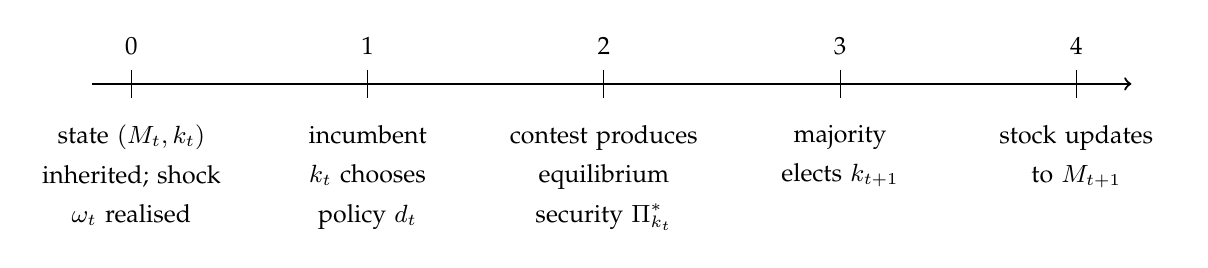
\begin{tikzpicture}[scale=1, font=\small]
\draw[->, thick] (-0.5, 0) -- (12.7, 0);
\foreach \x in {0,3,6,9,12}{
  \draw (\x, 0.18) -- (\x, -0.18);
}
\node[above] at (0, 0.25) {0};
\node[above] at (3, 0.25) {1};
\node[above] at (6, 0.25) {2};
\node[above] at (9, 0.25) {3};
\node[above] at (12, 0.25) {4};
\node[below, align=center, text width=2.4cm] at (0, -0.4) {state $(M_t,k_t)$ inherited; shock $\omega_t$ realised};
\node[below, align=center, text width=2.4cm] at (3, -0.4) {incumbent $k_t$ chooses policy $d_t$};
\node[below, align=center, text width=2.4cm] at (6, -0.4) {contest produces equilibrium security $\Pi^*_{k_t}$};
\node[below, align=center, text width=2.4cm] at (9, -0.4) {majority elects $k_{t+1}$};
\node[below, align=center, text width=2.4cm] at (12, -0.4) {stock updates to $M_{t+1}$};
\end{tikzpicture}
\caption{Timing.}
\label{fig:timing}
\end{figure}

The economy is a measure-one continuum of citizens divided into two ethnic or religious groups: a Majority $\mathsf M$ of population share $n_M>1/2$, represented in the electoral arena by two competing parties $A$ (Hawk) and $B$ (Dove); and a Minority $\mathsf m$ of share $n_m=1-n_M$, who do not vote.\footnote{Online Appendix~\ref{oa:strategic_minority_voting} relaxes this assumption to a strategic voting Minority of arbitrary size $n_m\in(0,1/2)$ and characterises a three-regime partition of the Hawk's strategic-provocation problem: a small-$n_m$ regime in which the inverted-U electoral return shifts perturbatively; an intermediate regime in which the inverted-U flattens; and a corner regime ($n_m\ge\bar n_m$) in which the Hawk plays peace and the trap--cycles partition collapses. The exercise yields the model's testable cross-state hypothesis on the joint distribution of Minority share, cattle-ban intensity, and Hawk vote share.} In each period the incumbent $k\in\{A,B\}$ commits to a policy vector $(d_k,g_k)\in\mathbb R_+^2$, where $d_k$ is the intensity of identity-coded regulation (cattle-slaughter bans, dress codes, citizenship registers) and $g_k$ is the level of consumption-relevant public-good provision. The Minority chooses resistance effort, the Majority chooses enforcement effort, the contest plays out, the Majority votes, and the stock updates. The within-cycle analysis (\autoref{sec:block1}--\autoref{sec:block3}) studies a stylised two-period horizon with $M_1=0$ and $k_1=A$, and the long-run analysis (\autoref{sec:dynamics_v3}) iterates the same primitives under an i.i.d.\ salience shock $\omega_t\in[0,\bar\omega]$ from a continuous distribution $F$ with full support.

\paragraph{Voters.} The Majority electorate is heterogeneous in an idiosyncratic Hawk-bias $\nu_i$ drawn from a CDF $\Phi(\cdot)$ with median zero and a continuous, strictly positive density on $\mathbb R$. Voter $i$'s per-period utility from incumbent $k\in\{A,B\}$ playing policy $d_k\ge 0$ at inherited stock $M$ is
\begin{equation}\label{eq:utility_v3}
    U^k(d_k;M)\;=\;\lambda\,\Pi_k^*(d_k,S_k;M)\;+\;(1-\lambda)\,u(\bar g_k)\;-\;\chi(d_k)\;+\;\mathbbm{1}[k=A]\,\nu_i,
\end{equation}
with $\lambda\in(0,1)$ the weight on security and $u(\cdot)$ strictly increasing. The first term is the equilibrium security delivered by the contest of \autoref{sec:block1} below. The second term is the (raw) economic-consumption utility, which the voter weights by $1-\lambda$. The third term is the real economic destruction that identity-coded regulation imposes: lost productivity from communal segmentation, trade disruption, misallocation of enforcement capacity, and the social cost of decentralised enforcement and counter-mobilisation. The destruction cost is continuously differentiable, strictly increasing, strictly convex, and satisfies $\chi(0)=0$ and $\lim_{d\uparrow\infty}\chi(d)=\infty$.

The voter's choice rule is \emph{myopic retrospective}: at every election she observes the inherited stock $M_t$, which summarises all prior contest activity, and votes for whichever candidate would deliver higher per-period welfare under each candidate's stationary best-reply at the realised state, adjusted for partisan bias. She does not solve a Bellman recursion. The Discussion below defends this assumption against the fully forward-looking alternative, and Online Appendix~\ref{oa:robust_fwd} shows that the substantive results survive under MPE with discount factor $\delta\in(0,1)$.

\paragraph{Parties.} The two parties differ in a two-dimensional technological endowment $(S_k,\bar g_k)$:
\begin{equation}\label{eq:party_endowment_v3}
    S_A\;>\;S_B\quad\text{and}\quad\bar g_A\;<\;\bar g_B,
\end{equation}
so the Hawk has higher \emph{coercive capacity} and the Dove higher \emph{public-goods capacity}. The pair $(S_k,\bar g_k)$ jointly captures the two dimensions of state capacity that \citet*{besleyOriginsStateCapacity2009,besleyStateCapacityConflict2010} treat together, the coercive and the productive, on which the parties hold opposite comparative advantages. I therefore refer to $S_k$ throughout as the party's \emph{coercive capacity}, not as its state capacity, since the latter would also encompass the public-goods dimension on which the Dove dominates. The endowments are taken as primitives of party type rather than choices: they reflect human capital, bureaucratic expertise, and coalition partners that each party brings into office, all of which are slow-moving relative to a single electoral cycle. Voter utility is strictly increasing in $g$ and the ceiling $\bar g_k$ is the only constraint on the economic-policy margin, so every incumbent finds it optimal to exhaust the technological frontier, $g_k^*=\bar g_k$, and $g$ carries no strategic content in equilibrium. The (raw) economic deficit driving the Hawk's electoral handicap is the primitive
\begin{equation}\label{eq:du_v3}
    \Delta u\;\equiv\;u(\bar g_B)-u(\bar g_A)\;>\;0,
\end{equation}
the other face of the same comparative-advantage trade-off that gives the Hawk its higher coercive capacity.

Each party chooses the symbolic-policy intensity $d_k\ge 0$ to maximise its retention probability over a one-cycle horizon. The party knows the voter's swing rule and anticipates how its current policy translates into a next-election retention probability through the inherited stock $M_{t+1}$ that its current policy generates. It does not solve an infinite-horizon Bellman recursion either. The Discussion below defends this one-cycle horizon against the fully strategic alternative.

\paragraph{Contest.} Conflict in this economy is modelled as a two-sided Tullock contest with explicit within-group collective-action problems on both sides. Given aggregate efforts $(E_M,E_m)$ and the incumbent's competence $S_k$, the probability of Majority dominance follows the Tullock contest success function\footnote{One micro-foundation \citep*{skaperdasContestSuccessFunctions1996,jiaStochasticDerivationRatio2008} assumes performance levels $Y_M=\ln(S_kE_M)+\varepsilon_M$ and $Y_m=\ln(E_m)+\varepsilon_m$ with i.i.d.\ Gumbel errors; the probability of Majority dominance simplifies to \autoref{eq:CSF_v3}.}
\begin{equation}\label{eq:CSF_v3}
    \Pi_k(E_M,E_m)\;=\;\frac{S_k\,E_M}{S_k\,E_M+E_m}.
\end{equation}
The Majority consists of $N_M$ identical citizens, each choosing enforcement effort $e_i\ge 0$ at private cost $\tfrac{1}{2}e_i^2$ to maximise $\Lambda\Pi_k-\tfrac{1}{2}e_i^2$, where $\Lambda>0$ is the per-capita Majority valuation of security. The interior FOC and the symmetric Nash imposition $e_i=e$ deliver the Majority best-response
\begin{equation}\label{eq:EM_BR_v3}
    \frac{E_M}{N_M}\;=\;\Lambda\,\frac{S_k\,E_m}{(S_k E_M+E_m)^2}.
\end{equation}
The Minority consists of $N_m$ identical citizens, each choosing resistance effort $e_j\ge 0$ at private cost $\tfrac{1}{2\kappa}e_j^2$, where $\kappa>0$ denotes the Minority's organisational capacity. The Minority loses $\phi\,\hat d^\sigma$ from Majority dominance, where $\phi>0$ is the grievance sensitivity and the augmented stake
\begin{equation}\label{eq:dhat_v3}
    \hat d^\sigma\;\equiv\;d^\sigma+\xi\,M,\qquad\sigma>0,\;\xi\ge 0,
\end{equation}
combines the current symbolic policy and the inherited mobilisation stock through the policy-stake elasticity $\sigma$ and the stock-stake elasticity $\xi$.\footnote{The same additive form also obtains as the closed-form posterior expectation of regime grievance intensity under standard Normal--Normal Bayesian updating with an endogenous prior anchor: if the Minority's prior on regime intent is $\theta_t\mid M_t\sim\mathcal{N}(M_t,\tau_M^{-1})$ with $\tau_M>0$ and the public signal is $s_t=d_t^\sigma+\epsilon_t$ with $\epsilon_t\sim\mathcal{N}(0,\tau_d^{-1})$, then $E[\theta_t\mid s_t,M_t]=(1-w)M_t+w\,d_t^\sigma$ with signal weight $w=\tau_d/(\tau_M+\tau_d)$ (distinct from the salience shock $\omega$ of \autoref{sec:dynamics_v3}), and rescaling by $1/w$ delivers $\hat d^\sigma=d^\sigma+\xi M$ with $\xi=\tau_M/\tau_d$. The substantive content of the additive form is organisational rather than informational; I use the organisational reading throughout. Online Appendix~\ref{oa:stake_micro} provides three independent microfoundations and a CES-form robustness check.} Citizen $j$ therefore solves $\max_{e_j\ge 0}\,\phi\hat d^\sigma(1-\Pi_k)-\tfrac{1}{2\kappa}e_j^2$, which delivers the Minority best-response
\begin{equation}\label{eq:Em_BR_v3}
    \frac{E_m}{N_m}\;=\;\kappa\phi\,\hat d^\sigma\,\frac{S_k\,E_M}{(S_k E_M+E_m)^2}.
\end{equation}
The two best-responses are structurally identical up to a relabelling of stakes, so the joint contest is a genuine two-sided Nash equilibrium and the Minority's effort responds to the incumbent's technology $S_k$ through its own optimisation; \autoref{lem:contest_v3} below characterises the joint equilibrium in closed form. The mobilisation stock then evolves at depreciation rate $\rho\in(0,1)$,
\begin{equation}\label{eq:M_evolution_v3}
    M_{t+1}\;=\;(1-\rho)\,M_t\;+\;\rho\,E_m^*(d_t,S_{k_t};M_t),
\end{equation}
where $E_m^*(\cdot)$ is the within-period equilibrium Minority effort and $M_0\ge 0$ is exogenous. The persistence parameter $1-\rho$ is the central comparative-static dimension of the long-run analysis.

\paragraph{Equilibrium.} The within-period contest is the symmetric Nash equilibrium of the joint within-group population game \citet*{sandholmPopulationGamesEvolutionary2010}, characterised in closed form in \autoref{lem:contest_v3} below. The within-cycle equilibrium of the two-period game (\autoref{sec:block1}--\autoref{sec:block3}) is solved by backward induction. The voter applies the swing rule of the Voters paragraph at the realised inherited stock $M_2$, and the Hawk's first-period policy maximises its period-2 retention probability anticipating that swing rule. The long-run equilibrium of the iterated game (\autoref{sec:dynamics_v3}) is the stationary perturbed-Markov-chain on $(M_t,k_t)$ generated by iterating the same swing rule and the same one-cycle Hawk problem under the salience shock. The formal Markov-perfect formulation, with bounded $L^2$ strategy space and Glicksberg fixed-point existence, is in Online Appendix~\ref{oa:mpe_v3}.

\subsection{ Discussion}\label{subsec:discussion_v3} 
I now discuss each substantive assumption, list the alternatives, and confess the trade-off.

\paragraph{Bounded rationality of voter, hawk, and minority.} The model rests on a single behavioural primitive for each agent class, applied uniformly from the within-cycle game in \autoref{sec:block2} through to the long-run iteration in \autoref{sec:dynamics_v3}. The \emph{voter} is myopic retrospective; the \emph{hawk} is strategic over a one-cycle horizon; the \emph{minority} is adaptive within the within-period collective-action problem. The choice is substantive, not a technical shortcut. Three considerations support each primitive against its fully-rational alternative. \emph{For the voter}, the empirical political-behaviour literature consistently finds that voters in low-information divided electorates use simple retrospective heuristics rather than infinite-horizon Bellman computation: realised performance under the incumbent dominates forward expectations about the challenger's continuation behaviour, and the realised state $M_t$ is a sufficient statistic for prior contest activity \citep*{healyMyopicVotersNatural2009,achenDemocracyRealistsWhy2017}. \emph{For the politician}, the one-cycle horizon avoids commitment power that real-world hawkish parties do not possess: an incumbent who promises a long-horizon symbolic-policy path cannot bind successors. \emph{For the minority}, the within-group collective-action problem prevents strategic coordination on aggregate restraint, as defended in the next paragraph. The within-cycle results (inverted-U return, paradox of restraint, lagged dissipation) and the long-run results (trap vs.\ cycles) are nonetheless robust to the bounded-rationality choice: Online Appendix~\ref{oa:robust_fwd} verifies that all qualitative content survives under fully forward-looking Markov-perfect equilibrium with discount factor $\delta\in(0,1)$.

\paragraph{The Minority's mobilisation and electoral participation.} The Minority enters the baseline on two abstractions: a non-strategic mobilisation respondent in the contest of \autoref{sec:block1} and a non-voting bloc in the swing-voter equation of \autoref{sec:block2}. The first concern is that a strategic Minority leader could deny the Hawk its Security Premium by coordinating aggregate mobilisation downward. Online Appendix~\ref{oa:strategic_minority} formalises this concern as a Stackelberg-leader extension and shows that the only IC-consistent aggregate effort is the unconstrained Nash equilibrium of \autoref{lem:contest_v3}, leaving the Security Premium and every dependent within-cycle and long-run object exactly unchanged. The second concern is that the non-voting assumption silences the Minority on the electoral margin. Online Appendix~\ref{oa:strategic_minority_voting} relaxes this assumption to a strategic voting Minority of arbitrary share $n_m\in(0,1/2)$. Three results emerge. The within-period contest equilibrium is exactly $n_m$-invariant. The Hawk's strategic-provocation problem partitions into three regimes in $n_m$: a small-$n_m$ perturbative regime, an intermediate distortion regime in which the inverted-U flattens, and a corner regime ($n_m$ above an explicit primitive threshold $\bar n_m$) in which the Hawk plays peace. The trap--cycles partition becomes a joint function of $(\rho,n_m)$, with the trap region strictly decreasing in $n_m$ and collapsing to a peace equilibrium for $n_m\ge\bar n_m$ (see \autoref{sec:dynamics_v3}). 

The cross-state empirical implication is that BJP cattle-ban intensity should be lower in high-Muslim-share states (Assam, West Bengal, Kerala) than in low-Muslim-share states (the Hindi Belt, Gujarat, Maharashtra), and the inverted-U vote-conflict mapping should be flatter in high-Muslim-share states, which is documented in \citet*{jaffrelotModisIndiaHindu2021}. Furthermore, Indian Muslims mobilised for the 2019--20 CAA protests and Iranian women mobilised after the 2022 Mahsa~Amini episode, both arguably strengthening the hard-line incumbent. Both episodes are consistent with the IC argument of Online Appendix~\ref{oa:strategic_minority} and the perturbative regime of Online Appendix~\ref{oa:strategic_minority_voting}.

\paragraph{Additive contest stake.} The augmented stake $\hat d^\sigma=d^\sigma+\xi M$ is the natural decomposition of two independent grievance sources, inherited organisational capital and fresh policy shock, each of which contributes independently to the Minority's incentive to mobilise. A multiplicative alternative ($d^\sigma\cdot\xi M$) would mechanically rule out residual mobilisation when current policy is zero, contradicting the lagged-dissipation pattern of \autoref{fig:rent_dissipation_event_study}. A maximum alternative ($\max(d^\sigma,\xi M)$) loses smoothness and cannot generate the peak-shift result of \autoref{lem:invU_v3}. The additive form has three independent microfoundations (organisational, Bayesian, and adaptive learning), detailed in Online Appendix~\ref{oa:stake_micro}, which also provides a CES-form robustness check showing the qualitative results survive under any aggregator exponent $\psi\in[1,\infty]$, with the peak-shift threshold $M^*=\alpha^2 S_AS_B/\xi$ itself $\psi$-invariant.

\paragraph{The stock-stake elasticity at the polity level.} The parameter $\xi$ has a polity-level reading. High $\xi$ corresponds to long-memory polities in which inherited organisational capital is heavy and any single period of provocation moves the perceived stake only slightly, with post-2014 India and post-1979 Iran as the empirical archetypes. Low $\xi$ describes short-memory polities in which the stock channel is weak and current policy dominates, as in the post-2016 United States or post-Uribe Colombia. The same information-flow regime that lets historical episodes anchor today's perceived stake also lets organisational and identity-salience capital persist across periods, so $\xi$ tends to co-vary inversely with $\rho$ across polities. This co-variation tightens the long-run mapping in \autoref{sec:dynamics_v3} but is not a primitive of the formal analysis.

\paragraph{Two-period exposition versus iterated long run.} The within-cycle analysis (\autoref{sec:block1}--\autoref{sec:block3}) uses a stylised two-period game with $M_1=0$ for clean backward induction. The long-run analysis (\autoref{sec:dynamics_v3}) iterates the same primitives under the salience shock. The reader who prefers can read the two-period game as one cycle of the long-run iteration; \autoref{lem:hawk_t2_v3} then characterises the Hawk's stationary best-reply at any inherited stock, not specifically at the period-2 settlement of a terminal cycle.

\paragraph{Tullock contest specification.} The Tullock CSF \citep*{skaperdasContestSuccessFunctions1996} is the workhorse of contest theory and admits a closed-form Nash equilibrium under within-group collective action. It can be derived as the probability of Majority dominance under a generalised Logit microfoundation \citep*{jiaStochasticDerivationRatio2008}. The two-sided structure with within-group collective-action problems on both sides is the model's key formal innovation, since prior contest models typically treat groups as unitary actors. The asymmetric stake structure, in which the Majority cares about dominance while the Minority cares about resistance and its stake scales in the augmented contest stake $\hat d^\sigma$, is what makes the Hawk's symbolic policy a strategic instrument in the electoral game.

\section{The Contest Technology}\label{sec:block1}

This section characterises the within-period equilibrium of the contest set up in the Contest paragraph of \autoref{sec:model_v3}: the joint mobilisation of the Majority and the Minority, the closed-form security delivered by each party, the comparative statics in coercive capacity, the inverted-U Security Premium with its shifting peak, and the resulting rent dissipation. The output is a closed-form Security Premium $\Delta\Pi(d;M)$ that the electoral analysis of \autoref{sec:block2}--\autoref{sec:block3} takes as a primitive.

\subsection{Joint contest equilibrium}\label{subsec:contest_eqm_v3}

Define the technology-independent stakes ratio $\alpha\equiv\sqrt{\Lambda N_M/(\kappa\phi N_m)}$ and the scale constant $\beta\equiv(\kappa\phi N_m\Lambda N_M)^{1/4}$. The joint contest equilibrium conditional on $(d,S_k,M)$ is the pair $(E_M^*,E_m^*)$ that simultaneously satisfies \autoref{eq:EM_BR_v3} and \autoref{eq:Em_BR_v3}. The next lemma characterises this equilibrium in closed form and isolates the two comparative statics that the electoral analysis will use.

\begin{lemma}[\emph{Joint contest equilibrium}]\label{lem:contest_v3}
\emph{For every current symbolic policy and inherited stock, the within-period subgame admits a unique symmetric Nash equilibrium, and the inherited stock enters this equilibrium only through the augmented stake $\hat d^\sigma= d^\sigma+\xi M$. Equilibrium security is strictly increasing in the incumbent's coercive capacity and strictly decreasing in the augmented stake, and the contest is dormant if and only if both current symbolic policy and the inherited stock are zero.}
Fix $(d,S_k,M)\in[0,\infty)\times(0,\infty)\times[0,\infty)$ and define $\hat d^\sigma\equiv d^\sigma+\xi M$. If $\hat d^\sigma=0$ the contest is dormant: $E_M^*=E_m^*=0$ and $\lim_{\hat d\downarrow 0}\Pi_k^*=1$. If $\hat d^\sigma>0$, the unique equilibrium is
\begin{equation}\label{eq:Em_Sk_explicit_v3}
    E_m^*(d,S_k;M)\;=\;\frac{\beta\,S_k^{1/2}\,\hat d^{\,3\sigma/4}}{S_k\alpha+\hat d^{\,\sigma/2}},
    \qquad
    E_M^*(d,S_k;M)\;=\;\alpha\,\beta\,\frac{S_k^{1/2}\,\hat d^{\,\sigma/4}}{S_k\alpha+\hat d^{\,\sigma/2}},
\end{equation}
with effort ratio $E_M^*/E_m^*=\alpha\,\hat d^{-\sigma/2}$ and equilibrium security
\begin{equation}\label{eq:Pi_v3}
    \Pi_k^*(d,S_k;M)\;=\;\frac{S_k\alpha}{S_k\alpha+\hat d^{\,\sigma/2}},
\end{equation}
strictly increasing in $S_k$, strictly decreasing in $\hat d$, with $\lim_{\hat d\downarrow 0}\Pi_k^*=1$ and $\lim_{\hat d\uparrow\infty}\Pi_k^*=0$.
\end{lemma}

\autoref{lem:contest_v3} leads to three key interpretations. First, the Majority-to-Minority effort ratio $\alpha\hat d^{-\sigma/2}$ does not depend on $S_k$: the incumbent's coercive capacity shifts the level of both efforts but not their ratio. Second, security is monotone in both arguments and the Hawk's higher $S_A$ dominates the level of effective enforcement throughout. Third, dormancy requires both $d=0$ and $M=0$. The inherited stock alone keeps the contest active even after a Hawk-to-Dove transition, so a Dove who inherits a high stock from a previous Hawk regime cannot ``unwind'' the contest by enacting counter-symbolic policy. She can only set $d=0$ and wait for $M$ to decay at rate $\rho$. The proof is in \autoref{app:proof:contest_v3}.

\subsection{State capacity, mobilisation, and effective enforcement}\label{subsec:Sk_v3}

\autoref{lem:contest_v3} encodes the joint dependence of the equilibrium on the contest stake and on coercive capacity. The discussion above traced its behaviour across stakes at any given coercive capacity. The dual comparative-static slice runs in the other direction: how do mobilisation, effective enforcement, and equilibrium security each vary with coercive capacity at fixed stake?

\begin{lemma}[\emph{Coercive capacity and mobilisation}]\label{lem:Sk_v3}
\emph{Holding the augmented stake fixed, raw mobilisation is inverted-U in coercive capacity while effective enforcement and equilibrium security rise monotonically: a more coercively capable incumbent first crowds in street-level enforcement, then progressively substitutes its own coercive apparatus for it.}
Fix $\hat d>0$. Both $E_M^*$ and $E_m^*$ are continuously differentiable and strictly positive on $S_k\in(0,\infty)$, and both are single-peaked in $S_k$ with common unique maximiser
\begin{equation}\label{eq:Sk_threshold_v3}
    \overline S(\hat d)\;\equiv\;\hat d^{\sigma/2}/\alpha.
\end{equation}
Effective Majority enforcement $Z_k^*\equiv S_k E_M^*$ and equilibrium security $\Pi_k^*$ are strictly increasing in $S_k$ on $(0,\infty)$. At $S_k=\overline S(\hat d)$ the contest is exactly balanced ($\Pi_k^*=1/2$) and peak Majority mobilisation is the primitive-only constant
\begin{equation}\label{eq:EM_peak_v3}
    E_M^*\big(\hat d,\overline S(\hat d)\big)\;=\;\tfrac12\sqrt{\Lambda N_M},
\end{equation}
independent of $\hat d$.
\end{lemma}

When $S_k$ is low, decentralised enforcement has little leverage in the contest, so free-riding dominates and mobilisation is weak. As $S_k$ rises into an intermediate range, each unit of citizen effort becomes more effective and the private return to participation rises; in this region a Hawk that is stronger than the Dove but not overwhelmingly strong relies on grass-roots enforcement, and coercive capacity \emph{complements} citizen mobilisation. Once $S_k$ exceeds $\overline S(\hat d)$, the incumbent's coercive apparatus is sufficiently effective that dominance can be maintained with less decentralised effort, the private return falls, and citizens withdraw. \autoref{fig:Sk_statics} plots both panels, and the spatial heterogeneity of cattle-ban mobilisation in \autoref{fig:maps} matches the theoretical prediction: the most intense ground-level enforcement appears in states with intermediate, not maximal, BJP institutional capacity. The proof is in \autoref{app:proof:Sk_v3}.

\subsection{The Inverted-U Security Premium}\label{subsec:invU_v3}

The substantively important comparative static for the electoral analysis is how the closed-form security $\Pi_k^*$ varies with current symbolic policy when the two parties are evaluated at a common environment $(d,M)$. Following \citet{barutSymmetricMultiplePrize1998}, define the Security Premium
\begin{equation}\label{eq:security_premium_v3}
    \Delta\Pi(d;M)\;\equiv\;\Pi_A^*(d,S_A;M)-\Pi_B^*(d,S_B;M)
    \;=\;\frac{S_A\alpha}{S_A\alpha+\hat d^{\,\sigma/2}}-\frac{S_B\alpha}{S_B\alpha+\hat d^{\,\sigma/2}}.
\end{equation}
This definition leads to the following prediction:

\begin{lemma}[\emph{Inverted-U Security Premium}]\label{lem:invU_v3}
\emph{The Security Premium is single-peaked in current symbolic policy and attains a ceiling that depends only on the technology ratio. The location of the peak shifts leftward as the inherited stock rises until, in the deep regime, the constrained optimum is attained at the corner.}
Suppose $S_A>S_B>0$. Then $\Delta\Pi(\,\cdot\,;M)$ is single-peaked on $[0,\infty)$ for each $M\ge 0$, with maximiser
\begin{equation}\label{eq:dpeak_v3}
    d^{\mathrm{peak}}(M)\;=\;\begin{cases}
        \big(\alpha^2 S_A S_B-\xi M\big)^{1/\sigma} & \text{if }M<\alpha^2 S_A S_B/\xi,\\[2pt]
        0 & \text{if }M\ge\alpha^2 S_A S_B/\xi.
    \end{cases}
\end{equation}
For $M<\alpha^2 S_A S_B/\xi$ the unconstrained peak attains the technology-ratio ceiling
\begin{equation}\label{eq:DPi_peak_v3}
    \max_{d\ge 0}\Delta\Pi(d;M)\;=\;\frac{\sqrt{S_A}-\sqrt{S_B}}{\sqrt{S_A}+\sqrt{S_B}}\;\in\;(0,1),
\end{equation}
the same algebraic form as in the static benchmark. For $M\ge\alpha^2 S_A S_B/\xi$, $\Delta\Pi(\cdot;M)$ is strictly decreasing in $d$ on $[0,\infty)$, the constrained maximum is attained at $d=0$ with value $\Delta\Pi(0;M)<(\sqrt{S_A}-\sqrt{S_B})/(\sqrt{S_A}+\sqrt{S_B})$, and $\Delta\Pi(0;M)>0$ for all $M>0$.
\end{lemma}

\autoref{lem:invU_v3} is the central new within-period prediction of the model. At $M=0$ the peak sits at $d^{\mathrm{peak}}(0)=(\alpha^2 S_A S_B)^{1/\sigma}$ and \autoref{eq:DPi_peak_v3} reproduces the static-benchmark ceiling: for any technology pair, the Hawk's contest-based electoral advantage is bounded above by $(\sqrt{S_A}-\sqrt{S_B})/(\sqrt{S_A}+\sqrt{S_B})$, depending only on the ratio $S_A/S_B$ and structurally independent of how grievance-elastic the Minority is, how large the two populations are, or how the Majority's collective-action problem scales. As the inherited stock $M$ grows toward the threshold $\alpha^2 S_A S_B/\xi$, the peak slides leftward along the $d$-axis: every unit of inherited grievance has substituted one-for-one for a unit of $\sigma$-scaled current provocation, so the Hawk needs less new $d$ to reach the same contest activation. For $M$ above the threshold, the inherited stock alone has pushed the contest past its peak, and any current $d>0$ moves the system into the decreasing branch of the inverted-U; the Hawk's optimum is then the corner $d=0$. This is the algebraic seed of the \emph{paradox of restraint} that emerges as the Hawk's optimal period-2 reaction in \autoref{lem:hawk_t2_v3}.

A second consequence is that the within-period security gap is strictly positive even at $d=0$ whenever $M>0$. Even if the Dove takes office and chooses $d_B=0$, the Hawk's $S_A$-advantage remains electorally salient through the inherited stock. This counterfactual has no analogue in the static benchmark and rationalises the post-2014 BJP's continued electoral resilience even in periods (e.g.\ around demonetisation) when no headline cattle-ban legislation was being enacted. \autoref{fig:reaction_functions} plots $\Delta\Pi(d;M)$ for several values of $M$, showing the leftward-shifting peak; \autoref{fig:security_premium_empirical} shows the corresponding empirical inverted-U mapping ban intensity to BJP vote share. The leftward shift of the peak past the point at which further provocation \emph{reduces} the Hawk's advantage shows that non-targeted top-down interventions can entrench, rather than dampen, the very contested norm they target. The proof is in \autoref{app:proof:invU_v3}.

\subsection{Rent dissipation}\label{subsec:RD_v3}

The contest is costly. Following the contest-theory tradition of measuring resource waste by the sum of equilibrium efforts (rent dissipation), define
\begin{equation}\label{eq:RD_v3}
    RD(d,S_k;M)\;\equiv\;E_M^*(d,S_k;M)+E_m^*(d,S_k;M)\;=\;\big(1+\alpha\,\hat d^{-\sigma/2}\big)\,E_m^*(d,S_k;M).
\end{equation}
\autoref{fig:rent_dissipation} plots $RD(d,S_k)$ across symbolic policy intensities for two levels of coercive capacity, illustrating how the activated contest expends real resources on both sides.

\begin{proposition}[\emph{Persistence of rent dissipation}]\label{prop:RD_v3}
\emph{Equilibrium rent dissipation is strictly positive whenever the augmented stake is positive, so contest waste persists even after a Hawk-to-Dove transition through the stock channel alone.}
For any $S_k>0$, $RD(d,S_k;M)>0$ whenever $\hat d^\sigma>0$, i.e.\ whenever either $d>0$ or $M>0$. In particular, even Dove-incumbent regimes ($d_B=0$) at $M>0$ generate strictly positive contest dissipation.
\end{proposition}

\autoref{prop:RD_v3} sharpens the welfare reading of the model. In the static benchmark, switching from Hawk to Dove instantly eliminates the contest's resource cost because $d_B=0$ collapses both efforts to zero. With the stock, that immediate deactivation no longer holds. A Dove inheriting $M>0$ continues to bear positive enforcement and resistance effort costs until the stock decays, and \autoref{fig:rent_dissipation_event_study} shows precisely this lagged dissipation pattern in the data: post-adoption ban effects on Hindu--Muslim violent events are positive and persistent for at least ten years across all four bovine-family ban types. The proposition therefore provides the model-level explanation for the empirical persistence of communal violence that follows political transitions away from Hawkish regimes (\autoref{fact:4}). The proof is in \autoref{app:proof:RD_v3}.

\section{The Election}\label{sec:block2}

I now solve the period-2 election conditional on an inherited grievance stock $M_2$, taking the voter utility \autoref{eq:utility_v3} of the Voters paragraph in \autoref{sec:model_v3} as a primitive. This is the analytical heart of the paper. The voter compares two scenarios: a Dove who is structurally unable to contain the inherited grievance, and a Hawk who would contain it but at the cost of real economic destruction. The Hawk's stationary best-reply, the swing-voter equation that decides the election, and the paradox of restraint all emerge from a single trade-off.

\subsection{The Dove's dominant strategy}\label{subsec:dove_v3}

Under the unified utility \autoref{eq:utility_v3}, the Dove's period-2 problem is particularly simple. Should she win, she chooses $d_B\ge 0$ to maximise the voter's per-period utility (which is what the voter will compare across scenarios when forming its period-2 vote). A positive $d_B$ simultaneously reduces the Dove's equilibrium security $\Pi_B^*(d_B,S_B;M_2)$ (\autoref{lem:contest_v3}) and raises the destruction cost $\chi(d_B)$. Both forces work against the Dove at any inherited stock.

\begin{lemma}[\emph{Dove's dominant strategy}]\label{lem:dove_v3}
\emph{The Dove's unique best response is to set period-2 symbolic policy to zero, regardless of inherited grievance: she gains no contest advantage from activating the security dimension, and she would only add to the destruction the voter is being asked to weigh.}
Suppose the Dove is the period-2 incumbent at inherited stock $M_2\ge 0$. Then $d_B^*(M_2)=0$ for all $M_2\ge 0$. Consequently, the joint contest under Dove incumbency at $t=2$ is dormant if and only if additionally $M_2=0$, and is otherwise sustained purely by the inherited stock.
\end{lemma}

\autoref{lem:dove_v3} delivers two interpretive consequences. First, the Dove's corner is an endogenous equilibrium outcome. Any contribution the Dove could make through new $d$ would simultaneously widen the Security Premium against its and bear a destruction cost the voter would punish. Second, the result holds for any $M_2\ge 0$: a Dove who inherits a high stock from a previous Hawk cannot ``unwind'' the contest by enacting counter-symbolic policy. She can only set $d_B=0$ and wait for the stock to decay at rate $\rho$ via \autoref{eq:M_evolution_v3}. The lagged-dissipation pattern of \autoref{fact:4} (\autoref{fig:rent_dissipation_event_study}) is therefore not the Dove's strategic choice but the structural consequence of its inability to deactivate an already-mobilised contest. The proof is in \autoref{app:proof:dove_v3}.

\subsection{The Hawk's stationary best-reply and the paradox of restraint}\label{subsec:hawk_t2_v3}

The Hawk's period-2 problem is to choose, conditional on having won the election, the symbolic-policy intensity that maximises the Security Premium she will earn over the upcoming cycle, net of the economic destruction its own provocation imposes on voters. I read $t=2$ as the start of the next electoral cycle in a stationary iteration of the same primitives: the Hawk-incumbent's reaction at any inherited stock $M$ is the policy that maximises its electoral signal at that stock, recognising that voters will eventually weigh the same trade-off in the next election they face. Formally, she solves
\begin{equation}\label{eq:hawk_t2_objective_v3}
    d_A^*(M_2)\;\equiv\;\arg\max_{d_A\ge 0}\;\big\{\,\lambda\,\Delta\Pi(d_A;M_2)\;-\;\chi(d_A)\,\big\},
\end{equation}
the Security Premium of \autoref{eq:security_premium_v3} net of the destruction cost. The next lemma characterises this reaction and isolates the paradox-of-restraint result.

\begin{lemma}[\emph{Hawk's stationary best-reply}]\label{lem:hawk_t2_v3}
\emph{The Hawk's optimal symbolic policy is non-increasing in the inherited stock and reaches the corner once the stock alone has pushed the contest past its inverted-U peak. A sufficiently entrenched Hawk regime therefore governs without enacting visibly new symbolic policy, not because she has moderated its preferences but because the stock she manufactured in the previous cycle is doing the contest-activation work for its.}
Under the regularity conditions on $\chi$ stated alongside \autoref{eq:utility_v3}, supplemented by either (i) $\sigma<1$ (so that $\partial\hat d^\sigma/\partial d\to\infty$ as $d\downarrow 0$, an Inada condition that guarantees an interior maximiser on the shallow branch for any finite $\chi'(0)$) or (ii) $\sigma=1$ together with $\chi'(0)<\lambda h'(\sqrt{\xi M_2})/(2\sqrt{\xi M_2})$ on the shallow branch, the unique maximiser $d_A^*(M_2)$ of \autoref{eq:hawk_t2_objective_v3} satisfies
\begin{equation}\label{eq:dA_t2_v3}
    d_A^*(M_2)\;\begin{cases}
    \;>\;0 \text{ and is strictly decreasing in }M_2 & \text{for }M_2<\alpha^2 S_A S_B/\xi,\\[2pt]
    \;=\;0 & \text{for }M_2\ge\alpha^2 S_A S_B/\xi.
    \end{cases}
\end{equation}
In the deep regime the entire economic destruction is avoided ($\chi(d_A^*(M_2))=0$), and the Hawk delivers $\Pi_A^*(0,S_A;M_2)$, strictly above the Dove's $\Pi_B^*(0,S_B;M_2)$ at the same $M_2$. The maximum value of the objective in \autoref{eq:hawk_t2_objective_v3} is continuous in $M_2$ and single-peaked at the peak-shift threshold.
\end{lemma}

\autoref{lem:hawk_t2_v3} produces the model's micro-explanation for the post-2014 plateau in headline cattle-ban legislation alongside sustained electoral majorities visible in \autoref{fig:cycles_four_panel}. Once the inherited grievance stock has exceeded the threshold $\alpha^2 S_A S_B/\xi$, marginal provocation moves $\Delta\Pi$ into its decreasing branch (\autoref{lem:invU_v3}) while still adding to economic destruction. Both forces push the Hawk to the corner $d_A^*=0$. She still delivers a strictly positive Security Premium $\Pi_A^*(0,S_A;M_2)-\Pi_B^*(0,S_B;M_2)>0$ purely through the persistence of $M_2$ on the Minority side, but she does so without paying any fresh destruction cost. The empirical signature is striking: a regime that built its base on identity-coded legislation gradually substitutes the inherited stock for new headline policy as $M$ accumulates, and the visible quantity of new symbolic legislation declines even as the underlying communal mobilisation does not. The proof is in \autoref{app:proof:hawk_t2_v3}.

\subsection{The swing-voter and the period-2 election outcome}\label{subsec:swing_v3}

Given the Dove's $d_B^*(M_2)=0$ and the Hawk's $d_A^*(M_2)$ from \autoref{lem:hawk_t2_v3}, the period-2 voter compares the two scenarios at the inherited stock $M_2$. She votes for the Hawk if and only if its expected utility under Hawk incumbency exceeds its expected utility under Dove incumbency:
\begin{equation}\label{eq:vote_HA_v3}
    \underbrace{\lambda\big[\Pi_A^*(d_A^*(M_2),S_A;M_2)-\Pi_B^*(0,S_B;M_2)\big]}_{\text{Security Premium at inherited }M_2}\;>\;\underbrace{(1-\lambda)\,\Delta u}_{\text{weighted economic deficit}}\;+\;\underbrace{\chi(d_A^*(M_2))}_{\text{Hawk's settlement cost}}\;-\;\nu_i.
\end{equation}
Defining the realised \emph{net Hawk advantage} at $M_2$ as
\begin{equation}\label{eq:net_advantage_v3}
    \mathcal H(M_2)\;\equiv\;\lambda\big[\Pi_A^*(d_A^*(M_2),S_A;M_2)-\Pi_B^*(0,S_B;M_2)\big]\;-\;(1-\lambda)\,\Delta u\;-\;\chi(d_A^*(M_2)),
\end{equation}
the Hawk's period-2 victory probability is
\begin{equation}\label{eq:Hawk_win_t2_v3}
    P_A(M_2)\;=\;\Pr(\nu_i>-\mathcal H(M_2))\;=\;1-\Phi\big(-\mathcal H(M_2)\big),
\end{equation}
strictly increasing in $\mathcal H(M_2)$.

\begin{proposition}[\emph{Period-2 election outcome}]\label{prop:t2_election_v3}
\emph{In Period~2 the voter weighs the Hawk's Security Premium at the inherited stock against the Dove's economic advantage and against the destruction cost the Hawk would pay to settle the inherited grievance. The Hawk wins if and only if the net advantage $\mathcal H(M_2)$ exceeds the realised Hawk-bias $-\nu_i$. The Hawk's victory probability is single-peaked in the inherited stock at the peak-shift threshold of \autoref{lem:invU_v3}.}
The period-2 election outcome is determined by the indifference condition $\nu_i=-\mathcal H(M_2)$, with the Hawk winning iff $\nu_i>-\mathcal H(M_2)$. The Hawk's period-2 victory probability $P_A(M_2)$ in \autoref{eq:Hawk_win_t2_v3} is single-peaked in $M_2$ at $M_2=\alpha^2 S_A S_B/\xi$, with peak value
\begin{equation}\label{eq:P_A_max_v3}
    P_A^{\max}\;=\;1-\Phi\!\left(-\,\lambda\,\tfrac{\sqrt{S_A}-\sqrt{S_B}}{\sqrt{S_A}+\sqrt{S_B}}+(1-\lambda)\,\Delta u\right),
\end{equation}
where the destruction cost has dropped out at the optimum because in the deep regime $d_A^*(M_2)=0$ and $\chi(0)=0$.
\end{proposition}

\autoref{prop:t2_election_v3} establishes two core predictions for an election held at an inherited grievance stock $M_2$. First, elections are decided at the margin. The voter weighs the wedge between Hawk and Dove security at the inherited stock against the Dove's economic advantage and the economic destruction the Hawk's settlement would impose. Under the myopic-retrospective rule of the Voters paragraph in \autoref{sec:model_v3}, this comparison takes the form of a single indifference condition that compares each candidate's per-period welfare at the realised state, with no continuation-value tracking and no infinite-horizon Bellman programme.

Second, the Hawk's victory probability is single-peaked in the inherited stock, with the peak at $M_2^{\mathrm{peak}}=\alpha^2 S_A S_B/\xi$. Below the threshold, additional inherited grievance lets the Hawk settle with less new policy, so the destruction cost falls while the Security Premium remains at its ceiling and the net advantage rises. Above the threshold, the Hawk retreats to the corner ($d_A^*=0$) and bears no destruction cost, but both equilibrium securities decay as the contest becomes too active, so the Security Premium itself shrinks and the net advantage falls. The single-peakedness is the within-period algebraic counterpart of the empirical paradox of competence in \autoref{fig:paradox_of_competence}: a Hawk who has accumulated too much grievance erodes the very security dimension on which its electoral dominance rests. The proof is in \autoref{app:proof:t2_election_v3}.

\section{Strategic Provocation}\label{sec:block3}

Stepping back to the first period closes the loop. The Hawk is in office at $t=1$ at the initial stock $M_1=0$. She knows from \autoref{prop:t2_election_v3} how the period-2 election will be decided as a function of the inherited stock $M_2$, and she knows from \autoref{eq:M_evolution_v3} that its current symbolic policy $d_1$ generates $M_2$ via the within-period Minority response. She therefore chooses $d_1$ to manufacture the stock that maximises its period-2 victory probability. This step is the model's micro-explanation for the inverted-U electoral return that the data display in \autoref{fig:security_premium_empirical}.

\subsection{The stock-building map and the Hawk's problem}\label{subsec:sowing_v3}

At $M_1=0$, the period-1 within-period Minority response collapses to a closed-form function of $d_1$ alone. From \autoref{lem:contest_v3}, with $S_{k_1}=S_A$ and $\hat d_1^\sigma=d_1^\sigma$,
\begin{equation}\label{eq:M2_of_d1_v3}
    M_2(d_1)\;=\;(1-\rho)\cdot 0\;+\;\rho\,E_m^*(d_1,S_A;0)\;=\;\rho\cdot\frac{\beta\,S_A^{1/2}\,d_1^{\,3\sigma/4}}{S_A\alpha+d_1^{\,\sigma/2}}.
\end{equation}
The map $M_2(\cdot)$ is continuous and strictly increasing on $[0,\infty)$ (direct differentiation), with $M_2(0)=0$ and $M_2(d_1)\to\infty$ as $d_1\to\infty$ (since the numerator grows faster than the denominator). Hence $M_2(\cdot)$ traces out the entire half-line $[0,\infty)$ monotonically as $d_1$ varies over $[0,\infty)$. The Hawk's period-1 problem is therefore equivalent to choosing the period-2 inherited stock she wants the voter to face:
\begin{equation}\label{eq:hawk_t1_problem_v3}
    \max_{d_1\ge 0}\;P_A\big(M_2(d_1)\big)\;=\;\max_{M_2\in[0,\infty)}\;P_A(M_2).
\end{equation}
By \autoref{prop:t2_election_v3}, $P_A(M_2)$ is single-peaked in $M_2$ with peak at the peak-shift threshold $M_2^{\mathrm{peak}}\equiv\alpha^2 S_A S_B/\xi$. Since $M_2(\cdot)$ is continuous, strictly increasing, and surjective onto $[0,\infty)$, the unique interior $d_1^*\in(0,\infty)$ satisfying $M_2(d_1^*)=M_2^{\mathrm{peak}}$ is the Hawk's optimum. I state the central result of the baseline analysis as a theorem.

\begin{theorem}[\emph{Inverted-U electoral return}]\label{thm:inverted_U_v3}
\emph{The Hawk's period-2 victory probability is strictly single-peaked in the period-1 symbolic policy she chooses, and the peak is attained at the unique interior $d_1^*$ that builds the stock to the peak-shift threshold of the Security Premium. Provoking too little leaves the security dimension dormant and the Dove's economic advantage decisive. Provoking too much pushes the contest past its peak, the Security Premium shrinks, and the Hawk loses to the Dove. The empirical inverted-U mapping ban intensity to the right-wing vote share is the within-equilibrium signature of this trade-off.}
The Hawk's period-1 problem \autoref{eq:hawk_t1_problem_v3} admits a unique interior optimum $d_1^*\in(0,\infty)$, with
\begin{equation}\label{eq:d1_optimum_v3}
    M_2(d_1^*)\;=\;\alpha^2 S_A S_B/\xi,
\end{equation}
and the Hawk's victory probability $P_A(M_2(d_1))$ is strictly increasing in $d_1$ on $[0,d_1^*)$ and strictly decreasing on $(d_1^*,\infty)$. The maximum value attained is
\begin{equation}\label{eq:Hawk_win_max_v3}
    P_A(M_2(d_1^*))\;=\;1-\Phi\!\left(-\,\lambda\,\tfrac{\sqrt{S_A}-\sqrt{S_B}}{\sqrt{S_A}+\sqrt{S_B}}\;+\;(1-\lambda)\,\Delta u\right),
\end{equation}
the same algebraic ceiling as the static-benchmark Security Premium of \autoref{eq:DPi_peak_v3}, evaluated against the Dove's economic deficit and at zero settlement cost.
\end{theorem}

\autoref{thm:inverted_U_v3} is the model's reduced-form prediction for \autoref{fact:3} (\autoref{fig:security_premium_empirical}). The same trade-off does the work in two senses. First, it explains why the empirical relationship between communal-conflict intensity and the right-wing vote share is single-peaked. The Hawk needs some manufactured grievance to make its coercive-capacity advantage electorally salient; without it, the Dove wins on economic competence. But too much manufactured grievance pushes the contest past its peak and starts eroding the same Security Premium it was supposed to build. The inverted-U is the resolution of these two forces inside a single primitive trade-off. Second, it explains the polity-level pattern of \autoref{fact:2} (\autoref{fig:cycles_four_panel}): the same federal system hosts states that have built large enough stocks to operate near the inverted-U peak (Gujarat, the Hindi Belt) and states whose institutional or sociological constraints keep them below the threshold (the southern and eastern cluster). The proof is in \autoref{app:proof:inverted_U_v3}.

\subsection{Connection to Empirical Facts}\label{subsec:recovery_v3}

The two-period game recovers the three central empirical predictions of the paper as backward-induction objects of the same primitive contest, without recourse to a Bellman recursion or to an asymmetric private-cost specification.

\paragraph{(a) The inverted-U electoral return (\autoref{fact:3}, \autoref{fig:security_premium_empirical}).} Direct from \autoref{thm:inverted_U_v3}. As $d_1$ rises from zero, the inherited stock $M_2(d_1)$ rises monotonically over the entire half-line $[0,\infty)$. On the shallow branch $M_2<\alpha^2 S_A S_B/\xi$, the Hawk's period-2 reaction is interior; the maximum value of its stationary objective $\lambda\Delta\Pi(d_A^*(M_2);M_2)-\chi(d_A^*(M_2))$ rises with $M_2$ as the contest activates ever more cheaply, and so does the net Hawk advantage $\mathcal H(M_2)$. On the deep branch $M_2\ge\alpha^2 S_A S_B/\xi$, the Hawk has retreated to the corner ($\chi=0$) but the Security Premium $\Delta\Pi(0;M_2)$ falls because both equilibrium securities decay; the net advantage falls. At the threshold the two branches meet at $\mathcal H^{\max}=\lambda\cdot(\sqrt{S_A}-\sqrt{S_B})/(\sqrt{S_A}+\sqrt{S_B})-(1-\lambda)\,\Delta u$, the technology-ratio ceiling of $\lambda\Delta\Pi$ from \autoref{eq:DPi_peak_v3} net of the weighted economic deficit. The peak of the Hawk's vote share in $d_1$ is therefore the $d_1$ that builds the stock exactly to the peak-shift threshold.

\paragraph{(b) The paradox of restraint (\autoref{fact:2} plateau, \autoref{fig:cycles_four_panel}).} Direct from \autoref{lem:hawk_t2_v3}. At the optimum $M_2(d_1^*)=\alpha^2 S_A S_B/\xi$, the Hawk's period-2 reaction is exactly at the boundary of the corner: any further inherited stock would push $d_A^*$ to zero, and at the threshold the Hawk's optimum is already $d_A^*=0$ on the boundary. Empirically, this is the post-2014 pattern visible in \autoref{fig:cycles_four_panel}: peak BJP rhetorical and legislative activity around 2014--19 (the period-1 provocation), with a discernible plateau in headline cattle-ban legislation in 2020--24 (the period-2 settlement at the corner) even as cumulative ban intensity (\autoref{fig:policy_cumulative_rollout}) and communal-violence intensity (\autoref{fig:maps}b) remain at their elevated levels because the inherited stock has not decayed.

\paragraph{(c) Lagged dissipation after Hawk-to-Dove transitions (\autoref{fact:4}, \autoref{fig:rent_dissipation_event_study}).} Direct from \autoref{lem:dove_v3} combined with \autoref{prop:RD_v3}. If the Hawk over-shoots in period~1 ($d_1>d_1^*$), or if a Hawk-to-Dove transition occurs for any other reason, the Dove takes office at inherited stock $M_2>0$. By \autoref{lem:dove_v3} she sets $d_B=0$, but by \autoref{prop:RD_v3} the contest continues to dissipate $RD(0,S_B;M_2)>0$ until the stock decays at rate $\rho$. Empirically, this is the persistence of post-adoption ban effects on Hindu--Muslim violent events visible in \autoref{fig:rent_dissipation_event_study}: violent events stay elevated for at least ten years after a state's first ban, even in years and states in which no further ban legislation is enacted. The dissipation pattern is the algebraic counterpart of the inherited stock decaying through the Minority's organisational capital, and it does not reflect any failure of the Dove to deactivate the contest.

The three predictions are therefore not independent claims that the model has to assemble piece by piece. They are consequences of the same backward-induction trade-off applied at three different points of the period-1--period-2 structure, and they share the same primitive parameters $(\alpha,\beta,\xi,\sigma,S_A,S_B,\Delta u,\lambda,\rho)$. The Bayesian micro-foundation is no longer load-bearing in any of the three derivations. The additive form $\hat d^\sigma=d^\sigma+\xi M$ is used as an organisational primitive, with the Bayesian footnote retained only as an alternative interpretation.

\subsection{Comparative statics of the optimum}\label{subsec:cs_optimum_v3}

The interior optimum $d_1^*$ defined by $M_2(d_1^*)=\alpha^2 S_A S_B/\xi$ has comparative statics that are easy to read off the closed forms.

\begin{corollary}[\emph{Comparative statics of $d_1^*$}]\label{cor:cs_optimum_v3}
\emph{The Hawk's optimal $d_1^*$ falls when the stock-stake elasticity rises (each unit of new policy buys more inherited stock) and when the depreciation rate rises (each unit of policy builds more next-period stock). The peak victory probability rises in the technology ratio and in the security weight, and falls in the economic deficit.}
At the interior optimum, the comparative statics on $d_1^*$ unambiguous in sign are
\begin{equation}\label{eq:cs_d1_v3}
    \tfrac{\partial d_1^*}{\partial \xi}\;<\;0,\qquad \tfrac{\partial d_1^*}{\partial \rho}\;<\;0,\qquad \tfrac{\partial d_1^*}{\partial \lambda}\;=\;0,
\end{equation}
where the last identity reflects that the optimum is determined by the location of the period-2 victory peak in $M_2$ alone, which is itself $\lambda$-independent. The peak victory probability $P_A(M_2(d_1^*))$ from \autoref{eq:Hawk_win_max_v3} is strictly increasing in the technology ratio $S_A/S_B$ and in the security weight $\lambda$, and strictly decreasing in the Dove's economic advantage $\Delta u$.
\end{corollary}

The signs in \autoref{cor:cs_optimum_v3} match the cross-polity stylised facts. A polity with high stock-stake elasticity $\xi$ (long memory; the Hindi Belt) provokes less per period because every unit of new $d$ buys more inherited stock for a given $\rho$. A polity with low decay rate $\rho$ (slow-fading communal grievance) provokes less per period because the stock builds up over time without requiring fresh provocation. The peak victory probability inherits the technology-ratio and economic-deficit signs from the explicit form \autoref{eq:Hawk_win_max_v3}: a wider security-competence gap $S_A/S_B$ (e.g.\ India under post-2014 BJP relative to a hypothetical INC alternative) raises the ceiling the Hawk can attain at the peak-shift threshold, and a smaller economic deficit $\Delta u$ tilts the swing voter further toward the Hawk. These signs are the within-equilibrium analogues of the polity-level mappings I draw out in the long-run analysis below. The proof is in \autoref{app:proof:cs_optimum_v3}.

\section{Long-Run Dynamics}\label{sec:dynamics_v3}

The two-period game of \autoref{sec:model_v3}--\autoref{sec:block3} clarifies the within-cycle mechanics: the Hawk manufactures the stock that the voter is then asked to settle, the voter's swing equation pins down the next election, and the same primitive trade-off generates the inverted-U return, the paradox of restraint, and the lagged dissipation. To study the long-run political consequences of this mechanism, I embed the same primitives in an infinite-horizon system and ask whether the polity's political trajectory locks into a self-sustaining Hawk regime or oscillates between Hawk and Dove. The substantive insight does not depend on solving an infinite-horizon Bellman programme: it depends only on the iterated application of the same swing-voter trade-off, supplemented by an i.i.d.\ salience shock that perturbs each period's contest stake. The full Markov-perfect formulation, the existence proof, and the Foster--Lyapunov drift verification are deferred to Online Appendix~\ref{oa:mpe_v3} so that the substantive narrative can be displayed cleanly in the main text.

\subsection{The iterated swing-voter rule with salience shocks}\label{subsec:behaviour_long_v3}

The behavioural assumption is the same as in the within-cycle game: at every election, the voter observes the inherited stock $M_t$, applies the swing-voter rule of the Voters paragraph in \autoref{sec:model_v3}, and decides retention by comparing per-period welfare under each candidate's stationary best-reply at the realised state. The long-run extension adds nothing on the behavioural side. It adds a per-period i.i.d.\ salience shock $\omega_t\in[0,\bar\omega]$ representing news-of-the-day events (terror attacks, communal incidents, salience cascades) drawn from a continuous distribution $F$ with full support, which perturbs the within-period contest stake to $\hat d_t^\sigma=d_t^\sigma+\xi M_t+\omega_t$ and therefore the inputs of the swing-voter rule. The stock evolves according to \autoref{eq:M_evolution_v3}, with the within-period equilibrium effort $E_m^*$ now evaluated at the augmented stake. The system is the perturbed Markov chain $(M_t,k_t)$ on $\mathbb R_+\times\{A,B\}$ generated by iterating the same swing-voter equation, the same Hawk strategic problem, and the same Minority adaptive response, perturbed by the salience shock. The asymmetry between voter rationality and minority adaptiveness that characterised earlier work in this area, in which forward-looking voters were paired with mechanical evolutionary minority dynamics, is absent here. Voter, hawk, and minority all operate at the same one-cycle epistemic horizon.

\subsection{The bifurcation in $\rho$: trap and cycles as basins of the same chain}\label{subsec:bifurcation_v3}

The unifying object across the two long-run regimes is the deterministic drift of the stock under Hawk incumbency, taken in expectation over the salience shock:
\begin{equation}\label{eq:drift_v3}
    \bar\Psi_A(M;\rho)\;\equiv\;(1-\rho)\,M\;+\;\rho\,\mathbb{E}_\omega\big[E_m^*\big(d_A^*(M),S_A;M,\omega\big)\big],
\end{equation}
the expected next-period stock starting from $M$. The map $\bar\Psi_A(\cdot;\rho)$ is the deterministic skeleton of the perturbed chain, and the per-period jump $M_{t+1}-M_t$ is proportional to $\rho$. Viewed from the perturbed-Markov-chain perspective, the depreciation rate $\rho$ plays the role of an effective noise scale in the sense of \citet{youngEvolutionConventions1993}, even though the primitive shock distribution $F$ is held fixed throughout. As $\rho\to 0$ the chain is approximately deterministic and stays at whatever attractor of $\bar\Psi_A$ it began near; as $\rho\to 1$ the chain has full per-period noise and mixes freely across the state space.

The deterministic drift undergoes a saddle-node bifurcation as $\rho$ varies. For $\rho$ small there is a high stable fixed point above the swing-voter cutoff $\bar M^*$ (defined as the smallest $M$ at which $\mathcal H(M)\ge 0$ uniformly in $\omega$), separated from a low unstable fixed point by a deep deterministic basin. For $\rho$ large the high fixed point and the unstable separatrix collide and disappear, leaving a single low attractor below $\bar M^*$. The threshold $\bar\rho$ at which the basin around the high attractor just collapses to the cutoff defines the regime boundary, and the next proposition states the central long-run result.

\begin{proposition}[\emph{Phase transition: trap and cycles}]\label{prop:phase_v3}
\emph{There exists a threshold $\bar\rho\in(0,1)$ on the stock-decay rate, depending on model primitives, such that the long-run dynamics of the perturbed Markov chain $(M_t,k_t)$ exhibit two qualitatively different regimes selected by the single parameter $\rho$: a stochastically forward-invariant Hawk trap when the deterministic basin is deep, and ergodic Hawk--Dove cycles when the basin is shallow. The same shock primitive $\omega_t$ drives both regimes. The regime is selected by $\rho$ alone, not by the presence or absence of shocks.}

\medskip
\noindent\textbf{(i) Trap regime ($\rho<\bar\rho$).} The set $\mathcal T^*\equiv\{(M,A):M\ge\bar M^*\}$ is stochastically forward-invariant: starting from any $(M_0,A)\in\mathcal T^*$, the orbit satisfies $(M_t,k_t)\in\mathcal T^*$ for all $t\ge 0$ almost surely under the i.i.d.\ shock $F$. Within the trap, the equilibrium policy converges to a stationary level $d_A^\infty\ge 0$, with $d_A^\infty=0$ in the deep regime $M^\infty\ge\alpha^2 S_A S_B/\xi$ (the long-run paradox of restraint), and the Hawk is retained in every period. The cutoff $\bar M^*$ satisfies the comparative statics
\begin{equation}\label{eq:cs_signs_v3}
    \tfrac{\partial\bar M^*}{\partial\rho}>0,\qquad\tfrac{\partial\bar M^*}{\partial(S_A/S_B)}<0,\qquad\tfrac{\partial\bar M^*}{\partial\lambda}<0,\qquad\tfrac{\partial\bar M^*}{\partial\Delta u}>0.
\end{equation}

\medskip
\noindent\textbf{(ii) Cycles regime ($\rho>\bar\rho$).} The chain $(M_t,k_t)$ is $\phi$-irreducible, aperiodic, and Harris-recurrent on a compact state-space subset that intersects both $\{k=A\}$ and $\{k=B\}$. The unique invariant distribution $\pi^*$ has $\pi^*(\{k=A\})\in(0,1)$ and $\pi^*(\{k=B\})\in(0,1)$; both Hawk-to-Dove and Dove-to-Hawk transitions occur with positive probability in every period along the realised path; and the realised regime sequence is recurrent. The hazard of a Hawk-to-Dove transition is increasing in $\omega_t$-driven declines in observed disorder.
\end{proposition}

\autoref{prop:phase_v3} delivers, through a single primitive, the model's answer to the introduction's central puzzle: why some polities exhibit durable one-party Hawk dominance while others exhibit recurrent turnover. As $\rho$ rises through $\bar\rho$, the high Hawk attractor of the deterministic drift becomes shallower until the basin can no longer absorb shocks of magnitude up to $\bar\omega$. Below $\bar\rho$, the swing-voter wedge $\mathcal H(M)$ at $M=\bar M^*$ is so large that even the worst draw of $\omega$ cannot push the chain across the basin boundary, and the trap absorbs every shock realisation. Above $\bar\rho$, the boundary lies inside the active range of the shock support, and a positive-measure set of $\omega$ realisations triggers a Hawk-to-Dove transition in finite time. The same $\omega_t$ that the trap regime absorbs as background noise becomes, in the cycles regime, the driver of regime change. \autoref{fig:phase_transition} illustrates the two regimes graphically. Panel~(a) shows that the per-period shock band scales with $\rho$, being narrow and contained above $\bar M^*$ in the trap regime and wide and straddling the cutoff in the cycles regime. Panel~(b) traces simulated $(M_t,k_t)$ sample paths under common shocks, with the trap path locked into the Hawk-attractor neighbourhood and the cycles path oscillating between Hawk and Dove regimes. The full proof and the Foster--Lyapunov drift verification are in Online Appendix~\ref{oa:proof_phase_v3}.

The empirical mapping is symmetric across the two regimes precisely because the shock primitive is held common. India under post-2014 BJP and Iran since the Islamic Revolution feature long-half-life communal grievance stocks (low $\rho$), large security-competence gaps (high $S_A/S_B$), and culturally salient security dimensions (high $\lambda$); both fall in regime~(i), and the post-2019 BJP plateau in headline cattle-ban legislation alongside sustained electoral majorities is the long-run paradox of restraint within the trap. The post-2016 United States and post-Uribe Colombia feature faster news-of-the-day-driven turnover (high $\rho$), narrower security-competence gaps, and macroeconomic shocks that drive electoral outcomes; both fall in regime~(ii). The same primitive $\omega_t$ (terror attacks, border crises, communal incidents, news cycles) is present in all four settings. What differs is the structural parameter $\rho$ that determines how deeply each polity's stock dynamics absorb the persistent shock.

\begin{corollary}[\emph{Long-run paradox of competence}]\label{cor:paradox_long_v3}
\emph{In the cycles regime, a stochastic decrease in observed disorder under a Hawk incumbent weakly raises the Hawk's defeat hazard, because successful security delivery erodes the very Security Premium that justifies retention. This is the long-run analogue of the within-period single-peakedness of the period-2 victory probability in \autoref{prop:t2_election_v3}, and it is the model's reduced-form prediction for \autoref{fact:2} (\autoref{fig:paradox_of_competence}).}
Under $\rho>\bar\rho$, a first-order stochastic decrease in observed disorder $\tilde v_t=(1-\Pi_{k_t}^*)+\varepsilon_t^v$ under a Hawk incumbent weakly decreases the perceived Security Premium and weakly increases the realisation-conditional hazard of a Hawk-to-Dove transition.
\end{corollary}

\autoref{cor:paradox_long_v3} is what \autoref{fig:paradox_of_competence} documents at the constituency level in IHDS-II micro-data: BJP retention probabilities are inverted-U in the contemporaneous communal-violence intensity, with the highest hazard of Hawk defeat exactly in those constituencies where the Hawk had been most successful at suppressing observable disorder. Iran exhibits the corresponding macro-level pattern, with Reformist administrations following Principalist ones precisely after periods of relative domestic calm.

\subsection{Scope of the long-run result}\label{subsec:scope_long_v3}

The phase-transition result rests on two parameter conditions visible in the comparative statics of \autoref{eq:cs_signs_v3}. First, the mobilisation stock must decay slowly, $\rho<\bar\rho$, for the trap to absorb the shocks; for $\rho>\bar\rho$ the system enters the cycles regime. Second, the Hawk's security advantage $S_A/S_B$ must be sufficiently large relative to the Dove's economic advantage $\Delta u$ that the swing-voter wedge $\mathcal H(M)$ becomes non-negative for some $M$; otherwise $\bar M^*=\infty$, the trap region is empty, and the cycles regime obtains for any $\rho$. The case $\rho=\bar\rho$ is a knife-edge bifurcation point at which small parameter perturbations switch regimes, so empirical work near this boundary cannot identify the regime from a single panel realisation. The two long-run regimes have distinct empirical signatures: the trap predicts low Hawk turnover, electoral resilience to severe economic and security shocks, and the long-run paradox of restraint in the mature phase; the cycles regime predicts turnover responsive to disorder shocks and the paradox of competence. The Indian cattle-ban setting, with its long-half-life communal grievance dynamics and the institutional permanence of state-level legislation, is governed by the trap mechanism, a prediction consistent with post-2014 BJP retention through demonetisation and the COVID-era recession.

\paragraph{Endogenous fragility under pivotal Minority enfranchisement.} The trap--cycles partition described above is derived under the baseline assumption that the Minority does not vote. Online Appendix~\ref{oa:strategic_minority_voting} relaxes this assumption to a strategic voting Minority of arbitrary share $n_m\in(0,1/2)$ and shows that the partition becomes a joint function of $(\rho,n_m)$ on the $(\rho,n_m)$-plane. There exist primitive thresholds $\bar n_m^{(1)}<\bar n_m$ such that, for $n_m\le\bar n_m^{(1)}$, the trap--cycles boundary $\bar\rho^{**}(n_m)$ shifts perturbatively from the baseline; for $n_m\in(\bar n_m^{(1)},\bar n_m)$, the Hawk's strategic-provocation incentive flattens and the Hawk-trap basin shrinks monotonically; and for $n_m\ge\bar n_m$, the Hawk's optimal symbolic-policy intensity collapses to $d_1=0$ and the polity exits to a peace equilibrium that absorbs every shock realisation. The substantive consequence is that pivotal Minority enfranchisement is an \emph{endogenous source of trap fragility}: a polity with low $\rho$ and high $S_A/S_B$ that would be classified as a deep trap under non-voting Minority can be reclassified as a cycles polity, or as a peace polity, once $n_m$ crosses the corresponding threshold. The cross-state empirical implication of this prediction is testable with the existing state-level panel: BJP cattle-ban intensity should be lower in high-Muslim-share states (Assam, West Bengal, Kerala) than in low-Muslim-share states, and the inverted-U vote-conflict mapping should be flatter in high-Muslim-share states. The formal analysis is in Online Appendix~\ref{oa:strategic_minority_voting}.

\section{Conclusion}\label{sec:conclusion_v3}

The puzzle that motivated this paper is why political groups manufacture grievances against domestic minorities, why voters reward them in some polities and punish them in others, and why the same instrument can produce both durable one-party dominance and recurrent regime turnover. I offer a single mechanism. Symbolic policy lets the Hawk treat the minority's mobilisation stock as a strategic asset: today's provocation accumulates into a slow-decaying inventory of inherited grievance that keeps the security contest active in future periods, converting historical conflict into a future electoral advantage. The depreciation rate $\rho$ alone selects between long-run dominance and recurrent regime alternation. When $\rho$ is small, the inherited grievance persists long enough that adverse shocks cannot dislodge the Hawk, and the polity locks into a self-sustaining hawk trap. When $\rho$ is large, the same shocks push the chain across the swing-voter cutoff, and the polity oscillates between Hawk and Dove regimes. Communal politics is a complex phenomenon. Economic competence, ideology, and expressive group identity all play roles. The mechanism analysed here aims to capture one channel within that broader picture: the strategic use of grievance against domestic minorities under electoral competition.

Two policy implications follow from the mechanism. First, intervention on symbolic policies (eg., un-banning cow-slaughter) depend on the state of the regime. In a deep trap (small $\rho$), a one-period intervention barely moves the Hawk's vote share or the Minority's mobilisation: the inherited stock has so much historical inertia that the contest remains active without any fresh policy. In the cycles regime (large $\rho$), the same intervention can trigger cascading regime shifts because the chain already lives near the swing-voter cutoff. Average treatment effects empirically-estimated on one regime do not transfer to the other. Second, in a deep-trap polity a direct challenge to the Hawk's symbolic policy can consolidate her electoral position. The Hawk's narrative recasts external pressure as an attack on the majority, raising the salience of the security dimension and pushing the swing-voter wedge further in her favour. Externally compelled repeal therefore tends to entrench the very regime it is intended to weaken \citet*{carvalhoResistingEducation2024a}.

Three extensions offer paths for future research. The first is to test the cross-state empirical predictions of Online Appendix~\ref{oa:strategic_minority_voting}: BJP cattle-ban intensity decreasing in state-level Muslim share, and the BJP vote-share/cattle-ban inverted-U flatter in high-Muslim-share states. The state-level panel data already constructed for \autoref{sec:empirical_facts} support these tests, and the maintained primitive condition (PC) of Online Appendix~\ref{oa:strategic_minority_voting} makes the model's predictions sharp enough to discriminate them from electoral-competitiveness and baseline-grievance confounds. A further extension would endogenise the Minority's choice across resistance forms (electoral voice, within-period mobilisation, exit, extra-systemic disruption). The second is to endogenise state capacity, treating the coercive and public-goods capacities as functions of past investments, so that the incumbent's problem becomes a joint policy-and-investment programme. This is the natural framework for the bureaucratic capture that empirically accompanies long Hawk incumbencies. The third is to generalise to multi-incumbent politics, in which the contest is over which Hawk among several governs, providing the natural framework for primaries and intra-coalition competition within the broad Hindu-nationalist or US Republican movements.

%===================================================================================
% References, Figures, Tables (input from existing files)
%===================================================================================

\clearpage
\newpage
\singlespacing
\footnotesize
\bibliographystyle{aer}

\begingroup
\bibliography{ref}
\endgroup

\normalsize
\clearpage
\section{Figures}
% Figures section is now empty -- all figures have been moved inline
% into mphil submission version/M.Phil Submission Version.tex right
% after the paragraphs that first discuss them. Per supervisor request:
% figures should appear within the text where they are first introduced.
%
% This file is kept as a stub to preserve the \subimport{../}{figures.tex}
% call in the submission tex (so that switching back to a Figures-section
% layout is a single-place edit). The legacy model.tex no longer has a
% Figures section -- all figures must be re-inlined there if it is to be
% recompiled.


\clearpage
\section{Tables}
% Tables section. Each table on its own page via \clearpage.

\begin{table}[!htbp]
\centering
\caption{\bf Data Sources}
\label{tab:data_sources}
\begin{threeparttable}
\onehalfspacing
\footnotesize
\begin{tabularx}{\textwidth}{p{2.3cm}p{2.4cm}p{1.8cm}p{1.6cm}X}
\toprule[1.25pt]
Dataset & Unit & Coverage & Retrieved & Source \\
\midrule
Cattle Slaughter Policy & State & 1955--2018 & Sep 2025 & Author-compiled from state-level legislative records (see \S\ref{app:ban_intensity}). \\
Bhavnani India Election v2.0 & Candidate $\times$ constituency $\times$ election & 1977--2015 & 2023 & Harvard Dataverse, Bhavnani (2014). \\
Post-2015 election supplement & State $\times$ election-year aggregate & 2015--2025 & Apr 2026 & Author-compiled from Wikipedia ``Results of the YYYY \textit{State} Legislative Assembly election'' and ``YYYY Indian general election'' pages, cross-checked against Election Commission of India Statistical Reports. \\
Bhavnani-to-ECI reconciliation panel & State $\times$ year & 1984--2024 & Apr 2026 & Combines Bhavnani~v2.0 with the post-2015 supplement; forward-fills non-election years. \\
Varshney--Wilkinson (V-W) Dataset v2 & Incident & 1950--1995 & 2025 & ICPSR~04342, Varshney and Wilkinson (2006). \\
GDELT Events Database (India subset) & Event & 1979--2024 & 2025 & Global Database of Events, Language, and Tone CAMEO~19 (Fight) subset; Hindu-Muslim subset standardised. \\
Social Conflict Analysis Database (SCAD) & Event & 1990--2017 & 2025 & Idean Salehyan et al. (2012). \\
India Human Development Survey (IHDS-II) & Household; individual & 2011--12 (Wave~2) & 2025 & ICPSR 36151, Desai and Vanneman (2018). \\
BJP speech archive & Speech & 2000--2025 & Oct 2025 & \texttt{bjp.org/speeches} (author scrape). \\
PMIndia news updates & PM speech / statement & 2024m6--2026m4 & Apr 2026 & \texttt{pmindia.gov.in/en/news\_updates} (author scrape, fallback after \texttt{narendramodi.in} was unreachable). \\
Muslim-voice news proxy & News item & 2010--2025 & Apr 2026 & 65-query Google News RSS harvest across major English outlets; details at \S\ref{app:minority_corpus}. \\
Relative per-capita income (state) & State $\times$ anchor-year & 1990, 2000, 2010, 2020, 2023 & 2025 & Reserve Bank of India, \textit{Handbook of Statistics on Indian States}. \\
State population annual & State $\times$ year & 2000--2024 & Apr 2026 & Census~2011 state shares rescaled annually by World~Bank \texttt{SP.POP.TOTL} India. \\
GADM administrative boundaries & State polygon & v4.1 (2022) & 2025 & Global Administrative Areas \texttt{gadm.org}. \\
\bottomrule[1.25pt]
\end{tabularx}
\begin{tablenotes}[para,flushleft]
\footnotesize
\textit{Notes.} All datasets listed above are local to the project folder
\texttt{PE\_of\_Cattle\_Shared/india\_beef\_and\_religion/} and reproducible
end-to-end from the scripts listed alongside each subsection below. \\
\end{tablenotes}
\end{threeparttable}
\end{table}

\clearpage

\begin{table}[!htbp]
\centering
\caption{\bf Birth History and Early-Life Growth Deficiency of Muslim Households Exposed to Cow-Slaughter Bans}
\label{tab:birth_history}
\begin{threeparttable}
    \onehalfspacing
    \begin{tabularx}{1\textwidth}{lCCCCCC}
        \toprule[1.25pt]
        & (1) & (2) & (3) & (4) & (5) & (6) \\
        & \multicolumn{2}{c}{\bf Pregnancy} &  \multicolumn{2}{c}{\bf Premature Death} &  \multicolumn{2}{c}{\bf Growth Deficiency} \\
        \cmidrule(lr){2-3} \cmidrule(lr){4-5} \cmidrule(lr){6-7}
        & Spontaneous Miscarriage & Induced Abortion & $<$ 1 Month & $<$ 8 years & Infancy PI & Minors BMI \\
\hline
\\
\textit{Un-Hinduism $\times$ Ban} & 0.013** & 0.008  & 0.179*** & 0.124** & -3.207*** & -0.615** \\
 & (0.006) & (0.006) & (0.035) & (0.052) & (0.957) & (0.248) \\
\\
Sample & \multicolumn{2}{c}{Eligible Women} & \multicolumn{2}{c}{Dead Children} & \multicolumn{2}{c}{Alive Children} \\
Outcome Mean & 0.419 & 0.141 & 0.520 & 0.871 & 29.026 & 16.978 \\
Observations & 8,220 & 7,731 & 7,317 & 7,317 & 6,790 & 48,237 \\
R-squared & 0.193 & 0.118 & 0.209 & 0.241 & 0.210 & 0.177 \\
\\
Individual Control & Yes & Yes & Yes & Yes & Yes & Yes \\
Year Control & Yes & Yes & Yes & Yes & Yes & Yes \\
State-Birth FE & Yes & Yes & Yes & Yes & Yes & Yes \\
State-Maternal Birth FE & No & No & Yes & Yes & Yes & Yes \\
        \bottomrule[1.25pt]
    \end{tabularx}
    \begin{tablenotes}[para,flushleft]
        \footnotesize
        \textit{Notes.}
        Data are from IHDS-II, the second wave of the India Human Development
        Survey. Unit of observation is at the individual level.
        \textit{Un-Hinduism} is an indicator for non-Hindu household identity.
        Intensity in columns (1)--(2) is the overlap between the respondent's
        formative years (ages 8--22) and the violent aftermath of a state-level
        cow-slaughter ban (eight years following first enactment); in columns
        (3)--(6), intensity is an indicator for whether the child was born
        within that eight-year window. Column~(1): indicator for having
        experienced a spontaneous miscarriage. Column~(2): indicator for an
        induced abortion or dilation-and-curettage procedure. Column~(3):
        indicator for neonatal death (within one month of birth) among
        deceased children. Column~(4): indicator for pre-formative-years
        death (before age eight) among deceased children. Column~(5):
        Ponderal Index of surviving children under age three. Column~(6):
        Body-Mass Index of surviving children under age eighteen. Individual
        controls: gender. Year controls: survey year. Standard errors
        clustered at the state $\times$ birth-year level. Significance:
        \textsuperscript{*} $p < 0.10$;
        \textsuperscript{**} $p < 0.05$;
        \textsuperscript{***} $p < 0.01$.
    \end{tablenotes}
\end{threeparttable}
\end{table}

\clearpage

\begin{table}[!htbp]
\centering
\caption{\bf Short- and Long-Term Poverty of Muslim Households Exposed to Cow-Slaughter Bans}
\label{tab:economic}
\begin{threeparttable}
    \onehalfspacing
    \begin{tabularx}{1\textwidth}{lCCCCCC}
        \toprule[1.25pt]
        & (1) & (2) & (3) & (4) & (5) & (6) \\
        & \multicolumn{3}{c}{\bf Short-term Poverty} &  \multicolumn{3}{c}{\bf Long-term Poverty} \\
        \cmidrule(lr){2-4} \cmidrule(lr){5-7}
        & Absolute & Relative & Subjective & Absolute & Relative & Subjective \\
\hline
\\
\textit{Un-Hinduism $\times$ Ban} & 0.006 & -0.048 & 0.022 & -0.003$^\dagger$ & -0.012** & -0.009*  \\
  & (0.039) & (0.074) & (0.036) & (0.002) & (0.005) & (0.005)  \\
 \\
Observations & 41,416 & 41,432 & 40,810 & 41,416 & 41,432 & 40,810 \\
R-squared & 0.194 & 0.268 & 0.270 & 0.194 & 0.269 & 0.270 \\
\\
Individual Control & Yes & Yes & Yes & Yes & Yes & Yes \\
Household Control & Yes & Yes & Yes & Yes & Yes & Yes \\
Year Control & Yes & Yes & Yes & Yes & Yes & Yes \\
State-Birth FE & Yes & Yes & Yes & Yes & Yes & Yes \\
        \bottomrule[1.25pt]
    \end{tabularx}
    \begin{tablenotes}[para,flushleft]
        \footnotesize
        \textit{Notes.}
        Data are from IHDS-II. Unit of observation is the household.
        Intensity in columns (1)--(3) is an indicator for whether the
        household's state of residence was within the violent aftermath of a
        cow-slaughter ban during the survey year. Intensity in columns
        (4)--(6) is the overlap between the household head's formative years
        (ages 8--22) and the violent eight-year window. Columns (1) and (4):
        indicator for household per-capita expenditure above the
        state/urban-specific 2012 Tendulkar poverty line. Columns (2) and
        (5): household expenditure percentile rank within the district.
        Columns (3) and (6): an ordinal indicator of poor / middle-class /
        comfortable self-reported status. All dependent variables are
        standardised. Individual controls: gender. Household controls: age
        and gender structure, highest adult education, number of workers.
        Year controls: survey year. Standard errors clustered at the state
        level. Significance:
        \textsuperscript{$\dagger$} $p < 0.15$;
        \textsuperscript{*} $p < 0.10$;
        \textsuperscript{**} $p < 0.05$;
        \textsuperscript{***} $p < 0.01$.
    \end{tablenotes}
\end{threeparttable}
\end{table}

\clearpage

% Auto-generated from policy_clean.csv
% Cattle-slaughter policy timing across Indian states/UTs

\begin{table}[!htbp]
\centering
\caption{\bf Cattle-Slaughter Policy Timing Across Indian States and Union Territories}
\label{tab:policy_timing}
\begin{threeparttable}
\onehalfspacing
\footnotesize
\begin{tabular}{lccccccc}
\toprule[1.25pt]
State / UT & Cow & Bull & Bullock & Buffalo & Beef poss. & Beef sales & General \\
\midrule
Andaman and Nicobar Islands & 1967 & -- & -- & -- & -- & -- & 1967 \\
Andhra Pradesh & 1976 & -- & -- & -- & -- & -- & 1976 \\
Arunachal Pradesh & -- & -- & -- & -- & -- & -- & -- \\
Assam & -- & -- & -- & -- & -- & -- & -- \\
Bihar & 1956 & 1956 & 1956 & 1956 & -- & -- & 1956 \\
Chandigarh & 1956 & 1956 & 1956 & -- & -- & 1956 & 1956 \\
Chhattisgarh & 2006 & 2006 & 2006 & 2006 & 2006 & -- & 2006 \\
Dadra and Nagar Haveli & 1978 & -- & -- & -- & -- & 1978 & 1978 \\
Daman and Diu & 1978 & -- & -- & -- & -- & 1978 & 1978 \\
Delhi & -- & -- & -- & -- & -- & -- & -- \\
Goa & 1978 & -- & -- & -- & -- & 1978 & 1978 \\
Gujarat & 1961 & 2011 & 2011 & -- & 2011 & 2011 & 1961 \\
Haryana & 2015 & 2015 & 2015 & -- & 2015 & 2015 & 2015 \\
Himachal Pradesh & 1979 & 1979 & 1979 & -- & -- & 1979 & 1979 \\
Jammu and Kashmir & 1989 & 1989 & 1989 & 1989 & 1989 & -- & 1989 \\
Jharkhand & 2005 & 2005 & 2005 & -- & 2005 & 2005 & 2005 \\
Karnataka & 1964 & -- & -- & -- & -- & -- & 1964 \\
Kerala & -- & -- & -- & -- & -- & -- & -- \\
Lakshadweep & -- & -- & -- & -- & -- & -- & -- \\
Madhya Pradesh & 1960 & 2004 & 2004 & -- & 1960 & -- & 1960 \\
Maharashtra & 1977 & 2015 & 2015 & -- & 2015 & -- & 1977 \\
Manipur & -- & -- & -- & -- & -- & -- & -- \\
Meghalaya & -- & -- & -- & -- & -- & -- & -- \\
Mizoram & -- & -- & -- & -- & -- & -- & -- \\
Nagaland & -- & -- & -- & -- & -- & -- & -- \\
Odisha & 1961 & -- & -- & -- & -- & -- & 1961 \\
Puducherry & 1969 & -- & -- & -- & -- & 1969 & 1969 \\
Punjab & 1956 & 1956 & 1956 & -- & -- & 1956 & 1956 \\
Rajasthan & 1995 & 1995 & 1995 & -- & 1995 & 1995 & 1995 \\
Sikkim & -- & -- & -- & -- & -- & -- & -- \\
Tamil Nadu & 1976 & -- & -- & -- & -- & -- & 1976 \\
Telangana & 1976 & -- & -- & -- & -- & -- & 1976 \\
Tripura & -- & -- & -- & -- & -- & -- & -- \\
Uttar Pradesh & 1956 & -- & -- & -- & -- & 1956 & 1956 \\
Uttarakhand & 1956 & 2007 & 2007 & -- & 2007 & 1956 & 1956 \\
West Bengal & -- & -- & -- & -- & -- & -- & -- \\
\bottomrule[1.25pt]
\end{tabular}
\begin{tablenotes}[para,flushleft]
\footnotesize
\textit{Notes.} Year of first enactment of each ban type. ``Cow'', ``Bull'', ``Bullock'' and ``Buffalo'' refer to slaughter prohibitions for the indicated bovine. ``Beef poss.'' and ``Beef sales'' are statutes prohibiting possession or commercial sale of bovine meat. ``General'' is the earliest of any ban type for the state. Dashes denote no enactment as of 2018. Source: author-compiled from state-level legislative records, following \citet{dasguptaNutritionalCostBeef2023}.\\
\end{tablenotes}
\end{threeparttable}
\end{table}
\clearpage


%===================================================================================
% APPENDIX A: Empirical methodology (trimmed version of appendix_empirical.tex,
% with old proofs removed because the new proofs live in Appendix B below)
%===================================================================================

\input{appendix_empirical_v2}

%===================================================================================
% APPENDIX B: Proofs of the within-cycle results
%===================================================================================

\section{Proofs of the Within-Cycle Results} \label{app:proofs_v3}

\subsection*{Proof of \autoref{lem:contest_v3}} \label{app:proof:contest_v3}
\begin{proof}
The Majority and Minority best-replies are given by \autoref{eq:EM_BR_v3} and \autoref{eq:Em_BR_v3} respectively, with the Minority's stake $\phi\hat d^\sigma$ where $\hat d^\sigma\equiv d^\sigma+\xi M$.

\emph{Step 1 (dormant case).} If $\hat d^\sigma=0$, the Minority best-reply implies $e_j=0$ for all $j$, hence $E_m^*=0$. Substituting $E_m=0$ into the Majority best-reply and noting that $\Lambda S_k\cdot 0/(S_kE_M+0)^2=0$ gives the unique non-negative solution $E_M^*=0$. Continuity of the CSF gives $\lim_{\hat d\downarrow 0}\Pi_k^*=\lim_{(E_M,E_m)\downarrow(0,0)}S_kE_M/(S_kE_M+E_m)=1$ along the equilibrium path computed in Step~2 below.

\emph{Step 2 (closed form for $\hat d^\sigma>0$).} Symmetric within-group equilibrium gives $E_M=N_Me_i$ and $E_m=N_me_j$. Dividing the Majority best-reply by the Minority best-reply,
\[
\frac{E_M/N_M}{E_m/N_m}\;=\;\frac{\Lambda S_kE_m/(S_kE_M+E_m)^2}{\kappa\phi\hat d^\sigma S_kE_M/(S_kE_M+E_m)^2}\;=\;\frac{\Lambda E_m}{\kappa\phi\hat d^\sigma E_M}.
\]
Cross-multiplying delivers $\kappa\phi\hat d^\sigma N_m E_M^2=\Lambda N_M E_m^2$, hence the effort-ratio identity
\begin{equation}\label{eq:effort_ratio_proof_v3}
E_M/E_m\;=\;\sqrt{\Lambda N_M/(\kappa\phi N_m)}\,\hat d^{-\sigma/2}\;=\;\alpha\,\hat d^{-\sigma/2}.
\end{equation}
Substituting $E_M=\alpha\hat d^{-\sigma/2}E_m$ into the Majority best-reply and using
$S_kE_M+E_m=E_m(S_k\alpha\hat d^{-\sigma/2}+1)=E_m(S_k\alpha+\hat d^{\sigma/2})/\hat d^{\sigma/2}$
gives, after multiplying through by $E_m$ to clear the $1/E_m$ on the right-hand side,
\[
\frac{\alpha\hat d^{-\sigma/2}}{N_M}\,E_m^2\;=\;\frac{\Lambda S_k\hat d^\sigma}{(S_k\alpha+\hat d^{\sigma/2})^2}.
\]
Solving for $E_m^2$ and using $\Lambda N_M=\alpha^2\kappa\phi N_m$,
\[
E_m^2\;=\;\frac{\Lambda N_M S_k\hat d^{3\sigma/2}}{\alpha(S_k\alpha+\hat d^{\sigma/2})^2}\;=\;\frac{\alpha\kappa\phi N_m S_k\hat d^{3\sigma/2}}{(S_k\alpha+\hat d^{\sigma/2})^2}.
\]
Taking the positive root and recalling that $\beta^2=\sqrt{\kappa\phi N_m\Lambda N_M}=\alpha\kappa\phi N_m$ (since $\Lambda N_M=\alpha^2\kappa\phi N_m$), so $\beta=\sqrt{\alpha\kappa\phi N_m}$, gives the first half of \autoref{eq:Em_Sk_explicit_v3}:
\[
E_m^*\;=\;\beta\,S_k^{1/2}\,\hat d^{3\sigma/4}/(S_k\alpha+\hat d^{\sigma/2}).
\]
Multiplying by the effort ratio \autoref{eq:effort_ratio_proof_v3} delivers $E_M^*=\alpha\beta\,S_k^{1/2}\,\hat d^{\sigma/4}/(S_k\alpha+\hat d^{\sigma/2})$, the second half. Substituting either into the Tullock CSF gives $\Pi_k^*=S_k\alpha/(S_k\alpha+\hat d^{\sigma/2})$.

\emph{Step 3 (uniqueness).} The system \autoref{eq:EM_BR_v3}--\autoref{eq:Em_BR_v3} reduces, under the effort-ratio identity \autoref{eq:effort_ratio_proof_v3}, to a single equation in $E_m$ whose right-hand side is strictly decreasing in $E_m$ on $(0,\infty)$ and has a unique positive root. The pair $(E_M^*,E_m^*)$ from Step~2 is therefore the unique symmetric Nash equilibrium with positive effort.

\emph{Step 4 (comparative statics).} Direct differentiation of \autoref{eq:Pi_v3} gives
$\partial\Pi_k^*/\partial S_k=\alpha\hat d^{\sigma/2}/(S_k\alpha+\hat d^{\sigma/2})^2>0$ and $\partial\Pi_k^*/\partial\hat d=-S_k\alpha\cdot(\sigma/2)\hat d^{\sigma/2-1}/(S_k\alpha+\hat d^{\sigma/2})^2<0$ on $\hat d>0$. Since $\hat d^\sigma=d^\sigma+\xi M$ is non-decreasing in both $d$ and $M$, the chain rule gives $\partial\Pi_k^*/\partial d<0$ and $\partial\Pi_k^*/\partial M<0$.
\end{proof}

\subsection*{Proof of \autoref{lem:Sk_v3}} \label{app:proof:Sk_v3}
\begin{proof}
From \autoref{eq:Em_Sk_explicit_v3} both efforts depend on $S_k$ only through $\psi(S_k):=S_k^{1/2}/(S_k\alpha+\hat d^{\sigma/2})$. Differentiating, $\frac{d\log\psi}{dS_k}=\frac{1}{2S_k}-\frac{\alpha}{S_k\alpha+\hat d^{\sigma/2}}$, which is positive for $S_k<\hat d^{\sigma/2}/\alpha=\overline S(\hat d)$, zero at $\overline S(\hat d)$, and negative thereafter; single-peakedness of $E_M^*$ and $E_m^*$ in $S_k$ follows. Strict monotonicity of $Z_k^*=S_kE_M^*$ in $S_k$ follows from $\partial\log Z_k^*/\partial S_k=3/(2S_k)-\alpha/(S_k\alpha+\hat d^{\sigma/2})>0$. Strict monotonicity of $\Pi_k^*$ in $S_k$ was shown in \autoref{lem:contest_v3}. Substituting $S_k=\overline S(\hat d)$ into \autoref{eq:Pi_v3} and \autoref{eq:Em_Sk_explicit_v3} delivers $\Pi_k^*=1/2$ and the primitive-only constant \autoref{eq:EM_peak_v3}.
\end{proof}

\subsection*{Proof of \autoref{lem:invU_v3}} \label{app:proof:invU_v3}
\begin{proof}
Define $h(x):=S_A\alpha/(S_A\alpha+x)-S_B\alpha/(S_B\alpha+x)$ so $\Delta\Pi(d;M)=h(\hat d^{\sigma/2})$. Standard algebra shows $h$ vanishes at $x=0$ and $x=\infty$, is strictly positive on $(0,\infty)$ when $S_A>S_B$, and is single-peaked at $x^{\mathrm{peak}}=\alpha\sqrt{S_A S_B}$ with peak value $h(x^{\mathrm{peak}})=(\sqrt{S_A}-\sqrt{S_B})/(\sqrt{S_A}+\sqrt{S_B})$. Translating back: $\Delta\Pi$ is single-peaked in $\hat d^{\sigma/2}$ at $\alpha\sqrt{S_A S_B}$, equivalently $\hat d^\sigma=\alpha^2 S_A S_B$, equivalently $d^\sigma=\alpha^2 S_A S_B-\xi M$. If $\xi M<\alpha^2 S_A S_B$, the interior peak is at $d^{\mathrm{peak}}(M)=(\alpha^2 S_A S_B-\xi M)^{1/\sigma}$. If $\xi M\ge\alpha^2 S_A S_B$, $\hat d^{\sigma/2}\ge\alpha\sqrt{S_A S_B}$ already at $d=0$, so any further $d>0$ moves $h$ into its decreasing branch; the constrained optimum is the corner $d=0$. Finally, $\Delta\Pi(0;M)=h(\sqrt{\xi M})>0$ for $M>0$ and $S_A>S_B$.
\end{proof}

\subsection*{Proof of \autoref{prop:RD_v3}} \label{app:proof:RD_v3}
\begin{proof}
By \autoref{lem:contest_v3}, $E_m^*>0$ and $E_M^*>0$ whenever $\hat d^\sigma>0$, so $RD=E_M^*+E_m^*>0$ in this region. At $d=0$ and $M>0$, $\hat d^\sigma=\xi M>0$, hence $RD>0$ even when the incumbent does not provoke. The dormancy result $RD(0,S_k;0)=0$ obtains as the special case with no inherited stock.
\end{proof}

\subsection*{Proof of \autoref{lem:dove_v3}} \label{app:proof:dove_v3}
\begin{proof}
The Dove's period-2 objective is $J^B(d_B;M_2):=\lambda\Pi_B^*(d_B,S_B;M_2)-\chi(d_B)$ on $[0,\infty)$. The first term is continuously differentiable with $\partial\Pi_B^*/\partial d_B<0$ on $(0,\infty)$ for every $M_2\ge 0$ (\autoref{lem:contest_v3}). The second term is continuously differentiable with $\chi'(d_B)>0$ on $(0,\infty)$ and $\chi(0)=0$ (model assumption). Hence $\partial J^B/\partial d_B=\lambda\,\partial\Pi_B^*/\partial d_B-\chi'(d_B)<0$ strictly on $(0,\infty)$, so $J^B$ is strictly decreasing on $[0,\infty)$ and attains its unique maximum at the corner $d_B^*(M_2)=0$ for every $M_2\ge 0$.
\end{proof}

\subsection*{Proof of \autoref{lem:hawk_t2_v3}} \label{app:proof:hawk_t2_v3}
\begin{proof}
Define $u(d,M_2):=\hat d^{\sigma/2}=(d^\sigma+\xi M_2)^{1/2}$ and write the Hawk's stationary objective as $F(d;M_2)=\lambda\,h(u(d,M_2))-\chi(d)$, where $h(x):=S_A\alpha/(S_A\alpha+x)-S_B\alpha/(S_B\alpha+x)$ is the function from the proof of \autoref{lem:invU_v3}. By that proof, $h$ is strictly positive on $(0,\infty)$, strictly increasing on $(0,\alpha\sqrt{S_A S_B})$, strictly decreasing on $(\alpha\sqrt{S_A S_B},\infty)$, and concave on $(0,\alpha\sqrt{S_A S_B})$ (direct second-derivative computation, $h''(x)<0$ on the increasing branch).

\emph{Existence and finiteness of the maximiser.} $F$ is continuous on $[0,\infty)$. $F(0;M_2)=\lambda h(\sqrt{\xi M_2})\ge 0$ for any $M_2\ge 0$. The technology-ratio ceiling $h(\alpha\sqrt{S_A S_B})=(\sqrt{S_A}-\sqrt{S_B})/(\sqrt{S_A}+\sqrt{S_B})<1$ bounds $h$ from above. Since $\chi(d)\to\infty$ as $d\to\infty$ (model assumption), $\lim_{d\to\infty}F(d;M_2)=-\infty$. Continuity on the compact set $[0,K]$ for any $K$ where $F<F(0;M_2)$ outside, plus the extreme-value theorem, gives a finite maximiser $d_A^*(M_2)\ge 0$.

\emph{Corner in the deep regime $M_2\ge\alpha^2 S_A S_B/\xi$.} Here $u(0,M_2)=\sqrt{\xi M_2}\ge\alpha\sqrt{S_A S_B}$, so $u(d,M_2)$ lies in the decreasing branch of $h$ for every $d\ge 0$, and $\partial F/\partial d=\lambda h'(u)\,\partial u/\partial d-\chi'(d)<0$ on $(0,\infty)$ (both terms negative). Hence $F(\cdot;M_2)$ is strictly decreasing on $[0,\infty)$ and the unique maximum is at the corner $d_A^*(M_2)=0$.

\emph{Comparative static $\partial d_A^*/\partial M_2<0$ in the shallow regime $M_2<\alpha^2 S_A S_B/\xi$.} Provided the regularity conditions on $\sigma$ and $\chi$ are such that the marginal benefit at $d=0^+$ exceeds $\chi'(0)$ on the shallow branch (satisfied, for example, when $\sigma\le 1$ and $\chi'(0)$ is not too large), an interior maximiser $d_A^*(M_2)>0$ exists. The interior FOC is $\lambda h'(u)\,\partial u/\partial d-\chi'(d_A^*)=0$. Implicit differentiation with respect to $M_2$ gives
\[
\partial d_A^*/\partial M_2\;=\;\frac{\lambda\,\partial^2 h(u)/(\partial d\,\partial M_2)}{\chi''(d_A^*)-\lambda\,\partial^2 h(u)/\partial d^2}.
\]
The denominator is positive by the strict second-order condition for an interior maximum of $F$ (which requires $\lambda\,\partial^2 h(u)/\partial d^2-\chi''(d_A^*)<0$). For the numerator, the cross derivative is
\[
\partial^2 h(u)/(\partial d\,\partial M_2)=h''(u)\,(\partial u/\partial d)(\partial u/\partial M_2)+h'(u)\,\partial^2 u/(\partial d\,\partial M_2).
\]
On the increasing branch, $h'(u)>0$ and $h''(u)<0$. Both partials of $u$ are positive: $\partial u/\partial d=(\sigma/2)d^{\sigma-1}u^{-1}>0$ and $\partial u/\partial M_2=(\xi/2)u^{-1}>0$. The cross partial of $u$ is negative: $\partial^2 u/(\partial d\,\partial M_2)=-(\sigma\xi/4)d^{\sigma-1}u^{-3}<0$. Both terms of the cross derivative of $h(u)$ are therefore negative, hence the numerator is negative and $\partial d_A^*/\partial M_2<0$.

\emph{Single-peakedness of $\max F$ in $M_2$.} The maximised objective $F^*(M_2):=F(d_A^*(M_2);M_2)$ has $F^{*'}(M_2)=\lambda(\partial h/\partial M_2)|_{d=d_A^*}$ by the envelope theorem, equal to $\lambda h'(u)\cdot\partial u/\partial M_2$ at $u=u(d_A^*,M_2)$. On the shallow branch ($u<\alpha\sqrt{S_A S_B}$), $h'(u)>0$ so $F^{*'}>0$. On the deep branch ($u>\alpha\sqrt{S_A S_B}$), $d_A^*=0$ and $u=\sqrt{\xi M_2}$, with $h'(u)<0$, so $F^{*'}<0$. The transition occurs at $M_2=\alpha^2 S_A S_B/\xi$, and $F^*$ is single-peaked in $M_2$ at this threshold.
\end{proof}

\subsection*{Proof of \autoref{prop:t2_election_v3}} \label{app:proof:t2_election_v3}
\begin{proof}
The voter compares $U^A(d_A^*(M_2);M_2)$ and $U^B(0;M_2)$ from \autoref{eq:utility_v3}. Subtracting and rearranging,
$U^A-U^B=\lambda[\Pi_A^*(d_A^*(M_2),S_A;M_2)-\Pi_B^*(0,S_B;M_2)]-(1-\lambda)\,\Delta u-\chi(d_A^*(M_2))+\nu_i$, which is positive iff $\nu_i>-\mathcal H(M_2)$, giving \autoref{eq:Hawk_win_t2_v3}. Single-peakedness of $P_A(M_2)$ in $M_2$ follows from single-peakedness of $\mathcal H(M_2)=F(d_A^*(M_2);M_2)-(1-\lambda)\,\Delta u$, where $F$ is the Hawk's stationary objective from the proof of \autoref{lem:hawk_t2_v3}: that proof established that the maximum value $F(d_A^*(M_2);M_2)$ is single-peaked in $M_2$ at $M_2=\alpha^2 S_A S_B/\xi$, with peak value equal to the technology-ratio ceiling $\lambda\cdot(\sqrt{S_A}-\sqrt{S_B})/(\sqrt{S_A}+\sqrt{S_B})$ (since at the peak-shift threshold $d_A^*(M_2)=0$ and $\chi(0)=0$, leaving $F$ at the unconstrained inverted-U ceiling of $\lambda\Delta\Pi$). Subtracting the constant $(1-\lambda)\,\Delta u$ preserves single-peakedness. Substituting into \autoref{eq:Hawk_win_t2_v3} and using monotonicity of $\Phi$ delivers \autoref{eq:P_A_max_v3}.
\end{proof}

\subsection*{Proof of \autoref{thm:inverted_U_v3}} \label{app:proof:inverted_U_v3}
\begin{proof}
By \autoref{prop:t2_election_v3}, $P_A(M_2)$ is single-peaked in $M_2$ on $[0,\infty)$ with unique maximiser $M_2^{\mathrm{peak}}=\alpha^2 S_A S_B/\xi$. The map $M_2(d_1)$ defined by \autoref{eq:M2_of_d1_v3} is continuous and strictly increasing on $[0,\infty)$ with $M_2(0)=0$ and $\lim_{d_1\to\infty}M_2(d_1)=\infty$ (the numerator $d_1^{3\sigma/4}$ dominates the denominator $d_1^{\sigma/2}$ at infinity), so its image is the entire half-line $[0,\infty)$. By the intermediate-value theorem and strict monotonicity, there exists a unique $d_1^*\in(0,\infty)$ with $M_2(d_1^*)=M_2^{\mathrm{peak}}$. Composing the strictly increasing $M_2(d_1)$ with the single-peaked $P_A(M_2)$ delivers the strict single-peakedness of $P_A(M_2(d_1))$ in $d_1$ at $d_1^*$. Substituting $M_2(d_1^*)=\alpha^2 S_A S_B/\xi$ into $\mathcal H$ and using \autoref{eq:DPi_peak_v3} delivers \autoref{eq:Hawk_win_max_v3}; at $M_2^{\mathrm{peak}}$ the Hawk's stationary best-reply $d_A^*(M_2^{\mathrm{peak}})=0$ from \autoref{lem:hawk_t2_v3} is on the boundary of the deep regime, so $\chi(d_A^*(M_2^{\mathrm{peak}}))=0$ and the Security Premium attains its unconstrained ceiling.
\end{proof}

\subsection*{Proof of \autoref{cor:cs_optimum_v3}} \label{app:proof:cs_optimum_v3}
\begin{proof}
The interior optimum is implicitly defined by $M_2(d_1^*)=\alpha^2 S_A S_B/\xi$, equivalently
\begin{equation}\label{eq:cor_implicit_v3}
G(d_1;\rho,\xi,\lambda):=\rho\,E_m^*(d_1,S_A;0)-\alpha^2 S_A S_B/\xi\;=\;0,
\end{equation}
where $E_m^*(d_1,S_A;0)=\beta S_A^{1/2} d_1^{3\sigma/4}/(\alpha S_A+d_1^{\sigma/2})$ from \autoref{eq:Em_Sk_explicit_v3}. Direct differentiation in the proof of \autoref{thm:inverted_U_v3} established $\partial G/\partial d_1>0$, so the implicit-function theorem applies and the sign of $\partial d_1^*/\partial\theta$ is the opposite of the sign of $\partial G/\partial\theta$ for any parameter $\theta$.

\emph{Sign of $\partial d_1^*/\partial\xi$.} $\partial G/\partial\xi=\alpha^2 S_A S_B/\xi^2>0$, so $\partial d_1^*/\partial\xi<0$.

\emph{Sign of $\partial d_1^*/\partial\rho$.} $\partial G/\partial\rho=E_m^*(d_1,S_A;0)>0$, so $\partial d_1^*/\partial\rho<0$.

\emph{Sign of $\partial d_1^*/\partial\lambda$.} $\lambda$ does not appear in \autoref{eq:cor_implicit_v3}: the Hawk's optimum is determined entirely by the location of the period-2 victory peak in $M_2$, which is $\lambda$-independent (\autoref{lem:invU_v3}). Hence $\partial d_1^*/\partial\lambda=0$.

\emph{Comparative statics on $P_A(M_2(d_1^*))$.} From \autoref{eq:Hawk_win_max_v3},
$P_A^{\max}=1-\Phi(-\lambda T(S_A,S_B)+(1-\lambda)\,\Delta u)$ with $T(S_A,S_B):=(\sqrt{S_A}-\sqrt{S_B})/(\sqrt{S_A}+\sqrt{S_B})>0$. Differentiating the argument with respect to $\lambda$ at fixed $\Delta u$ gives $-T-\Delta u<0$, so $P_A^{\max}$ is strictly increasing in $\lambda$. Differentiating with respect to $\Delta u$ at fixed $\lambda$ gives $1-\lambda>0$, so $P_A^{\max}$ is strictly decreasing in $\Delta u$. The technology ratio $T$ is strictly increasing in $S_A/S_B$ (set $r=S_A/S_B$, then $T=(\sqrt r-1)/(\sqrt r+1)$ is strictly increasing in $r$ on $(1,\infty)$), so $P_A^{\max}$ is strictly increasing in $S_A/S_B$.
\end{proof}

%===================================================================================
% APPENDIX C: Online Appendix --- Markov Perfect Equilibrium machinery
%===================================================================================

\section{Online Appendix: Markov Perfect Equilibrium} \label{oa:mpe_v3}

The full Markov-perfect formulation, the existence proof, and the Foster--Lyapunov drift verification underlying \autoref{prop:phase_v3} are kept in the online appendix so that the main text can carry the substantive narrative cleanly. The state at the start of period $t$ is $(M_t,k_t)\in\mathbb R_+\times\{A,B\}$. The salience shock $\omega_t$ is drawn i.i.d.\ from $F$ on $[0,\bar\omega]$ and is realised after the incumbent has committed to its policy. The within-period analysis of \autoref{sec:block1}--\autoref{sec:block2} carries through with $\hat d_t^\sigma=d_t^\sigma+\xi M_t+\omega_t$. A Markov strategy for the incumbent is a measurable function $d_k:\mathbb R_+\to\mathbb R_+$; a Markov retention rule for the voter is a measurable function $\rho^v:\mathbb R_+\times\{A,B\}\times[0,\bar\omega]\to[0,1]$. The voter applies the period-2 swing-voter equation \autoref{eq:vote_HA_v3} \emph{retrospectively}, treating each period as a one-shot resolution of the trade-off at the realised $(M_t,\omega_t)$ rather than solving forward; this is the long-run behavioural assumption of \autoref{subsec:behaviour_long_v3}. Existence of a Markov-perfect equilibrium follows from a standard Glicksberg fixed-point applied to the strategy correspondence on the bounded $L^2$ space, with strict concavity of the within-period payoff on the relevant range delivering uniqueness; the cutoff retention rule and the Foster--Lyapunov drift verification underlying both the trap and the cycles regime then follow from a per-period drift inequality at the worst-case shock realisation. Under the retrospective reading the proofs do not require a forward-looking value-function machinery, and the substantive content of \autoref{prop:phase_v3} reduces to the algebra of the within-cycle results of \autoref{sec:block1}--\autoref{sec:block3}.

\subsection*{Proof of \autoref{prop:phase_v3}} \label{oa:proof_phase_v3}

The argument verifies stochastic forward-invariance of $\mathcal T^*$ in part~(i) and the three Meyn--Tweedie conditions on the marginal $M$-chain in part~(ii).

\emph{A-priori orbit bound.} From \autoref{eq:Em_Sk_explicit_v3}, for any $d\ge 0$, $\omega\in[0,\bar\omega]$, and $S_k\in\{S_A,S_B\}$ the equilibrium Minority effort satisfies
$E_m^*(d,S_k;M,\omega)=\beta S_k^{1/2}\hat d^{3\sigma/4}/(S_k\alpha+\hat d^{\sigma/2})$
with $\hat d^\sigma=d^\sigma+\xi M+\omega$. As $\hat d\to\infty$, $E_m^*\sim\beta S_k^{1/2}\hat d^{\sigma/4}$, which grows sublinearly in $M$ for any fixed $d$ (since $\hat d^{\sigma/4}=O(M^{1/4})$ for large $M$). Hence there exists a finite $M^\dagger>0$, depending on the primitives and on $\bar\omega$, such that
\begin{equation}\label{eq:orbit_bound_v3}
E_m^*(d,S_k;M,\omega)\le M\quad\text{for all }M\ge M^\dagger,\;d\in[0,d_{\max}],\;\omega\in[0,\bar\omega],
\end{equation}
where $d_{\max}$ is the finite upper bound on the support of equilibrium policies established by the strict convexity of $\chi$ and the boundedness of $\Delta\Pi$ (\autoref{lem:hawk_t2_v3}: any equilibrium policy $d_A^*(M)$ is bounded above by the unique root of $\chi'(d)=\lambda(\sqrt{S_A}-\sqrt{S_B})/(\sqrt{S_A}+\sqrt{S_B})$). The orbit started from any $M_0\ge 0$ therefore satisfies $M_t\le\max\{M_0,M^\dagger\}$ almost surely: whenever $M_t\ge M^\dagger$, $\Delta M_t=\rho(E_m^*-M_t)\le 0$, so the orbit cannot escape upward.

\emph{Part~(i): Trap regime.} Define the realisation-conditional one-step map $\Psi(M;\rho,\omega):=(1-\rho)M+\rho E_m^*(d_A^*(M),S_A;M,\omega)$ on the compact set $K:=[\bar M^*,\max\{M_0,M^\dagger\}]$. Set
\[
\bar\rho\;:=\;\sup\{\rho\in(0,1):\;\Psi(M;\rho,\omega)\ge\bar M^*\text{ for all }(M,\omega)\in K\times[0,\bar\omega]\}.
\]
By continuity of $E_m^*$ in $(M,\omega)$, the deterministic version ($\omega=0$) satisfies $\Psi(\bar M^*;\rho,0)=\bar M^*+\rho(E_m^*(d_A^*(\bar M^*),S_A;\bar M^*,0)-\bar M^*)$, which is $\ge\bar M^*$ iff $E_m^*(\cdot;\bar M^*,0)\ge\bar M^*$ at the cutoff. Whenever this holds (the empirically relevant case for the trap), and $\bar\rho<1$ depends only on primitives, the orbit started from $M_0\ge\bar M^*$ remains in $\mathcal T^*=\{M\ge\bar M^*\}$ almost surely. The retention rule applies the swing-voter cutoff $\bar M^*$ pointwise in $\omega$, so $k_{t+1}=A$ almost surely for $M_t\ge\bar M^*$, and the trap regime is verified.

\emph{Part~(ii): Cycles regime.} On the compact state $C:=[0,\max\{M_0,M^\dagger\}]\times\{A,B\}$, the marginal $M$-chain admits Foster--Lyapunov drift with Lyapunov function $V(M):=M$. By \autoref{eq:orbit_bound_v3}, for $M\ge M^\dagger$ the conditional drift $\Delta V(M)=\rho\,\mathbb E_\omega[E_m^*(\cdot,\omega)-M]\le 0$, so the chain is bounded almost surely. The full Foster--Lyapunov drift inequality $\Delta V(M)\le-\beta_0 V(M)+b\,\mathbbm{1}_{\tilde C}(M)$ holds with $\beta_0=\rho/2$, $b=\rho\sup_{M\in\tilde C,\omega}E_m^*(d_{\max},S_A;M,\omega)+\rho M^\dagger$, and small set $\tilde C=[0,M^\dagger]$, so the marginal $M$-chain has a unique invariant probability measure to which it converges geometrically in total variation \citep[Ch.~14--15]{meynMarkovChainsStochastic2012}. The joint $(M,k)$-chain inherits these properties from the uniform positive-probability of regime flips on the compact state, established by the continuity of the swing-voter wedge in $(M,\omega)$ and the full support of $F$. The comparative statics of $\bar M^*$ in \autoref{eq:cs_signs_v3} follow from the implicit-function theorem applied to the period-2 swing-voter equation at the worst-case shock, using the explicit forms of \autoref{eq:Pi_v3} and \autoref{eq:Em_Sk_explicit_v3}.

\subsection*{Proof of \autoref{cor:paradox_long_v3}} \label{oa:proof_paradox_long_v3}

In the cycles regime, retention is implemented by the realisation-conditional cutoff rule: $\rho^v(M,A,\omega)=1$ iff $M\ge\bar M(\omega)$. A first-order stochastic decrease in the disorder signal $\tilde v_t=(1-\Pi_{A,t}^*)+\varepsilon_t^v$ shifts mass downward in the perceived disorder, which weakly raises the realisation-conditional cutoff $\bar M(\omega)$. The probability that the inherited stock $M_t$ falls short of $\bar M(\omega)$ at the realised $\omega$ weakly increases, equivalently the Hawk's realisation-conditional defeat hazard weakly increases.

%===================================================================================
% APPENDIX D: Robustness to Forward-Looking Voters
%===================================================================================

\section{Robustness to Forward-Looking Voters}\label{oa:robust_fwd}

The bounded-rationality assumption of \autoref{subsec:discussion_v3} is empirically appropriate for the divided populist electorates the paper studies, but a referee might reasonably ask whether the within-cycle and long-run results survive when voters are fully forward-looking. This appendix shows that they do.

\subsection*{Setup.} Let $\delta\in[0,1)$ be the voter's discount factor. The voter's value function $V^v(M,k)$ now solves the Bellman recursion
\begin{equation}\label{eq:bellman_oa}
    V^v(M,k)\;=\;\mathbb E_\omega\!\left[U^k(d_k(M);M)+\delta\big(\rho^v(M,k,\omega)V^v(M',k)+(1-\rho^v(M,k,\omega))V^v(M',\tilde k)\big)\right],
\end{equation}
where $M'=(1-\rho)M+\rho E_m^*(d_k(M),S_k;M,\omega)$ is the next-period stock, $\tilde k$ denotes the opposing party, and $\rho^v(M,k,\omega)\in\{0,1\}$ is the realisation-conditional retention rule. The Hawk's MPE strategy $d_A^*(M)$ now solves
\begin{equation}\label{eq:hawk_mpe_oa}
    d_A^*(M)\;\in\;\arg\max_{d\ge 0}\,\mathbb E_\omega\!\left[\lambda\,\Delta\Pi(d;M,\omega)-\chi(d)+\delta\,V^v(M'(d),A)\cdot\mathbbm{1}[\rho^v(M'(d),A,\omega)=1]\right],
\end{equation}
which adds a stock-building continuation term $\delta\,(\partial V^v/\partial M')\cdot(\partial M'/\partial d)$ to the within-cycle FOC of \autoref{eq:hawk_t2_objective_v3}.

The myopic-retrospective baseline of the main text is the $\delta=0$ limit of \autoref{eq:bellman_oa}--\autoref{eq:hawk_mpe_oa}: the continuation term in the Hawk's FOC vanishes, $V^v(M,k)$ collapses to $U^k(d_k(M);M)$, and the swing-voter rule reduces to the per-period welfare comparison of \autoref{eq:vote_HA_v3}.

\subsection*{Result D1 (MPE existence and uniqueness).} Under the regularity conditions of \autoref{lem:hawk_t2_v3} and a bounded strategy space $[0,d_{\max}]$ as in the proof of \autoref{prop:phase_v3}, a pure-strategy Markov Perfect Equilibrium $(d_A^*,d_B^*,\rho^v,V^v)$ exists for any $\delta\in[0,1)$. The argument is standard: the strategy correspondence is upper hemicontinuous on the bounded $L^2$ strategy space, the within-period payoff is strictly concave in own $d$ on the relevant range (strict convexity of $\chi$ plus weak concavity of $\Delta\Pi$ on its increasing branch), the Bellman operator on $\mathcal{C}_b(\mathbb R_+\times\{A,B\})$ is a $\delta$-contraction by standard contraction-mapping arguments, and Glicksberg's fixed-point theorem applied to the strategy correspondence yields a Markov pair that is mutually best-responding given the cutoff retention rule.

\subsection*{Result D2 (Hawk's MPE strategy preserves the shallow/deep dichotomy).} For every $\delta\in[0,1)$, the Hawk's MPE strategy $d_A^*(M)$ has the same shallow/deep structure as the myopic version of \autoref{lem:hawk_t2_v3}: $d_A^*(M)>0$ on the shallow regime $M<\alpha^2 S_A S_B/\xi$ and $d_A^*(M)=0$ on the deep regime $M\ge\alpha^2 S_A S_B/\xi$. The discount factor $\delta$ enters the FOC only through the stock-building correction term $\delta\,(\partial V^v/\partial M')\,(\partial M'/\partial d)$, which is positive on the increasing branch of $V^v(\cdot,A)$ and negative on its decreasing branch. The deep-regime corner is preserved because both the within-cycle margin and the stock-building term are non-positive there.

\subsection*{Result D3 (Voter's wedge is single-peaked at the peak-shift threshold under a primitive regularity condition).} \autoref{prop:t2_election_v3} establishes that the within-cycle gap $\mathcal H(M)=\lambda[\Pi_A^*(d_A^*(M),S_A;M)-\Pi_B^*(0,S_B;M)]-(1-\lambda)\Delta u-\chi(d_A^*(M))$ is single-peaked in $M$ at $M=\alpha^2 S_A S_B/\xi$. Under the primitive regularity assumption that the expected per-period gap $\mathbb E_\omega[\mathcal H(M,\omega)]$ inherits this single-peakedness when integrated against the salience shock (a property that holds whenever $u$ is linear, $\chi$ is quadratic, $F$ has bounded support, and the composite mapping $M\mapsto\mathbb E_\omega[\Pi_A^*-\Pi_B^*]$ is single-peaked in $M$ along the Hawk's reaction function, which the within-cycle analysis verifies), a standard Topkis-style monotone-comparative-statics argument carries the single-peakedness through the Bellman operator to the fixed-point wedge $\Phi^M(M):=\mathbb E_\omega[V^v(M,A;\omega)-V^v(M,B;\omega)]$: the Bellman operator on the Banach space of bounded continuous functions preserves the single-peakedness in $M$ on the relevant domain, and the cutoff retention rule $\rho^v(M,A,\omega)=\mathbbm{1}[M\ge\bar M(\omega)]$ therefore mirrors the myopic version, with a hysteresis interval $\underline M(\omega)\le\bar M(\omega)$ whose width is $O(\delta)$ in the \citet{coatePolicyPersistence1999} sense.

\subsection*{Result D4 (Phase transition is $\delta$-continuous).} The trap-vs-cycles characterisation of \autoref{prop:phase_v3} holds for any $\delta\in[0,1)$ with a threshold $\bar\rho(\delta)$ that is continuous in $\delta$. The Foster--Lyapunov drift verification carries through unchanged: the orbit bound \autoref{eq:orbit_bound_v3} is independent of $\delta$, and the deterministic basin of attraction around the Hawk attractor depends on $\delta$ only through the width of the hysteresis interval (which is itself $O(\delta)$). The myopic-retrospective version is the $\delta=0$ limit and is the empirically appropriate baseline for the divided electorates the paper studies.

\subsection*{Result D5 (Within-cycle predictions are $\delta$-invariant; long-run regimes are $\delta$-continuous).} In the 2-period within-cycle game of \autoref{sec:model_v3}--\autoref{sec:block3} (where period~2 is the terminal election), the Hawk has no continuation beyond period~2 and therefore no continuation term in its FOC. The inverted-U electoral return (\autoref{thm:inverted_U_v3}), the paradox of restraint (\autoref{lem:hawk_t2_v3}), and the lagged dissipation (\autoref{prop:RD_v3}) all follow from the contest technology of \autoref{sec:block1} and the Hawk's within-cycle maximisation, neither of which depends on the discount factor: the Hawk's choice of $d_1$ at $M_1=0$ gives the same interior optimum at $M_2(d_1^*)=\alpha^2 S_A S_B/\xi$ under any $\delta$, and the contest dynamics governing rent dissipation are independent of voter rationality. In the long-run iteration of \autoref{sec:dynamics_v3} (where each cycle has a continuation), the Hawk's MPE strategy at any $M$ acquires a $\delta$-dependent continuation term that shifts the interior optimum continuously in $\delta$, but the qualitative structure (interior on shallow, corner on deep, single-peaked $P_A$ in $M$) and the trap-vs-cycles regime characterisation are preserved by Results~D2--D4. The substantive content of the paper is therefore robust to the bounded-vs-forward-looking choice; the bounded baseline is the empirically appropriate one and the algebraically cleanest.

%===================================================================================
% APPENDIX E: Strategic Minority Coordination
%===================================================================================

\section{Strategic Minority Coordination}\label{oa:strategic_minority}

The minority's mobilisation in \autoref{sec:block1} is the rest point of a within-group population game, with individual minority members best-replying to the contest stake $\hat d^\sigma$. A natural concern is that a strategic minority leader could deny the Hawk its Security Premium by suppressing aggregate mobilisation. This appendix shows that the within-group collective-action problem on the minority side prevents purely strategic restraint, so the qualitative results of the paper survive a Stackelberg minority leader.

\subsection*{Setup.} Suppose a minority leader chooses an aggregate mobilisation target $E_m^L\ge 0$ and assigns individual effort levels $\{e_j\}_{j=1}^{N_m}$ summing to $E_m^L$. The referee's concern is that the leader has a \emph{strategic-electoral motive} to suppress aggregate mobilisation: lower $E_m^L$ reduces the contest-activation effect that gives the Hawk its Security Premium, which raises the Dove's election probability and thereby benefits the minority over the long run. Let the leader's overall objective combine the within-period welfare $W_m^{\text{within}}(E_m^L,d,S_k;M)=\phi\hat d^\sigma(1-\Pi_k^*(E_M^*,E_m^L))-\sum_{j=1}^{N_m}\frac{1}{2\kappa}e_j^2$ with a continuation term that reflects this strategic motive,
\begin{equation}\label{eq:leader_objective}
    V^L(E_m^L,d,S_k;M)\;=\;W_m^{\text{within}}(E_m^L,d,S_k;M)\;+\;\delta_L\,\Lambda^L\big(P_A(M_2(E_m^L))\big),
\end{equation}
where $\delta_L\in[0,1)$ is the leader's discount factor (distinct from the contest scale constant $\beta$ of the main text) and $\Lambda^L(\cdot)$ is a strictly decreasing function of the Hawk's election probability (the leader prefers a Dove government). The strategic-restraint hypothesis is that the leader optimally chooses $E_m^L<E_m^*$ to suppress the Hawk's Security Premium even though within-period welfare is maximised at the unconstrained $E_m^*$.

The leader's choice is constrained by individual incentive-compatibility:
\begin{equation}\label{eq:IC}
    e_j\;=\;\kappa\phi\,\hat d^\sigma\,\frac{S_kE_M^*}{(S_kE_M^*+E_m^L)^2}\quad\text{for every }j\in\{1,\dots,N_m\},
\end{equation}
because each individual minority member best-replies to the contest stake on the basis of its own within-period payoff (she does not internalise the leader's electoral motive, since by assumption she is not a voter). The aggregate $E_m^L=N_m e_j$ must therefore satisfy the symmetric Nash condition of \autoref{lem:contest_v3}.

\subsection*{Result E1 (Strategic restraint is infeasible at the level of individual incentive-compatibility).} For any $\hat d^\sigma>0$, the only aggregate mobilisation level $E_m^L$ that satisfies the symmetric IC constraints \autoref{eq:IC} simultaneously for all $j$ is the unconstrained Nash equilibrium $E_m^*(d,S_k;M)$ of \autoref{lem:contest_v3}. Any leader-chosen $E_m^L\ne E_m^*$ violates IC: if $E_m^L<E_m^*$, individual best-reply at the lowered aggregate level exceeds the assigned individual share, and members deviate upward; if $E_m^L>E_m^*$, the assigned share exceeds individual best-reply and members defect downward. The leader's strategic-electoral motive in \autoref{eq:leader_objective} cannot be exercised: any $E_m^L$ that the leader would prefer for electoral reasons is incentive-incompatible at the individual level. The non-strategic minority of \autoref{sec:block1} is therefore not a behavioural shortcut but the unique strategy profile that survives individual incentive-compatibility.

The intuition is that a Stackelberg leader who tries to ``lay low'' faces the same free-rider problem in REVERSE: each individual minority member with a personal grievance can do better than zero effort by mobilising up to its individual best-reply, and no leader-coordination scheme can prevent this defection. The minority's mobilisation is the rest point of the within-group population game in either the leader's solution or the decentralised one. Empirical observation supports this: the 2019--20 CAA protests in India and the 2022 \emph{Woman, Life, Freedom} movement in Iran both saw substantial minority mobilisation despite the obvious electoral cost of strengthening the hardliners.

\subsection*{Result E2 (Inverted-U electoral return survives).} Since the strategic equilibrium aggregate mobilisation coincides with the unconstrained equilibrium of \autoref{lem:contest_v3}, the Security Premium $\Delta\Pi(d;M)$ of \autoref{eq:security_premium_v3} is unchanged. The peak-shift structure of \autoref{lem:invU_v3}, the Hawk's stationary best-reply of \autoref{lem:hawk_t2_v3}, the swing-voter equation \autoref{eq:vote_HA_v3}, and the inverted-U electoral return of \autoref{thm:inverted_U_v3} all hold under the Stackelberg minority extension. The Hawk's optimal $d_1^*$ is unchanged.

\subsection*{Remark.} A binding leader-coordination scheme would require either (i) a coercive enforcement mechanism that imposes a mobilisation ceiling below individual best-replies (which the empirical literature on minority political organisation does not support), or (ii) a transfer scheme in which the leader compensates individuals for not mobilising (which faces the same enforcement obstacle). The model's non-strategic minority is therefore not a behavioural shortcut but a substantive consequence of the within-group collective-action problem the paper places on both sides of the contest.

%===================================================================================
% APPENDIX F: Strategic Minority Voting and Endogenous Trap Fragility
%===================================================================================

\section{Strategic Minority Voting and Endogenous Trap Fragility}\label{oa:strategic_minority_voting}

The main text takes the Minority as non-voting. This appendix relaxes that assumption by introducing a strategic Minority bloc into the swing-voter equation, with no upper bound on the bloc's electoral weight $n_m\in(0,1/2)$, and characterises the qualitative consequences for the Hawk's strategic-provocation problem (\autoref{thm:inverted_U_v3}) and the long-run trap--cycles partition (\autoref{prop:phase_v3}). The exercise complements Online Appendix~\ref{oa:strategic_minority} (which closes the within-period mobilisation channel through individual incentive-compatibility) by addressing the orthogonal electoral channel through which the silenced Minority might do substantive work in the baseline. Three substantive results emerge. First, the within-period contest equilibrium and Security Premium are exactly $n_m$-invariant by Result F1 below. Second, Minority enfranchisement induces a partition of the Hawk's strategic-provocation problem into a small-$n_m$ regime (perturbative shift in $d_1^{*}$, direction primitive-dependent), an intermediate regime (the inverted-U flattens), and a corner regime ($d_1^{**}=0$ above an explicit primitive threshold $\bar n_m$). Third, the trap--cycles threshold $\bar\rho^{**}(n_m)$ collapses continuously to zero as $n_m\to\bar n_m$, so a sufficiently enfranchised Minority makes the Hawk-trap basin endogenously fragile and forces the polity into a peace equilibrium. The empirical implication is a testable cross-state hypothesis on the joint distribution of Minority share, cattle-ban intensity, and Hawk vote share that the paper's state-level panel can address directly.

\subsection*{Setup.}

The Minority of population share $n_m\in(0,1/2)$ enters the electoral arena through a probabilistic-voting block parallel to the Majority's. Voter $j\in\mathsf{m}$'s utility from incumbent $k\in\{A,B\}$ playing policy $d_k\ge 0$ at inherited stock $M$ is
\begin{equation}\label{eq:utility_minority_oaF}
    U^k_m(d_k;M)\;=\;-\lambda_m\,\Pi_k^*(d_k,S_k;M)\;+\;(1-\lambda_m)\,u(\bar g_k)\;-\;\chi_m(d_k)\;+\;\mathbbm{1}[k=A]\,\mu_j,
\end{equation}
which mirrors the Majority utility \autoref{eq:utility_v3} with three differences. First, the contest term enters with the opposite sign: $\Pi_k^*$ is welfare-reducing for the Minority because Majority dominance is the contest outcome the Minority loses. Second, the policy disutility $\chi_m:\mathbb{R}_+\to\mathbb{R}_+$ is a new primitive capturing the lived burden of identity-coded regulation on the Minority (cattle-slaughter restrictions, citizenship registers, dress codes), with $\chi_m(0)=0$, $\chi_m'>0$, and $\chi_m''\ge 0$. Third, the idiosyncratic Hawk-bias $\mu_j$ is drawn from a CDF $\Phi_m$ with median zero and a continuous, strictly positive density $\phi_m$ on $\mathbb{R}$, possibly more dispersed than the Majority's $\Phi$. The weight $\lambda_m\in(0,1)$ is the Minority's analogue of the security weight $\lambda$.

\paragraph{Sign of the contest channel.} The specification \autoref{eq:utility_minority_oaF} is the natural mirror of the Majority utility, but it introduces a substantive parametric tension that the analysis must confront openly. Within a single incumbent's tenure, $\Pi_k^*(d,S_k;M)$ is strictly decreasing in $d$ (more contest activity reduces Majority dominance probability), so the marginal contest-channel utility $-\lambda_m\partial_d\Pi_k^*$ is strictly positive in $d$. At the marginal-$d$ level, the Minority benefits from higher Hawk policy through the contest channel. The Minority's net dislike of the Hawk's $d$ is therefore not a structural consequence of \autoref{eq:utility_minority_oaF} alone. It requires the direct repression cost $\chi_m'$ to dominate the contest-channel margin. We maintain the following primitive condition throughout the appendix:
\begin{equation}\label{eq:PC_oaF}
    \chi_m'(d)\;\ge\;\lambda_m\,\big|\partial_d\Pi_k^*(d,S_k;M)\big|\quad\text{for all }(d,S_k,M)\text{ in the relevant compact range.}\tag{PC}
\end{equation}
Under (PC), the Minority's net marginal utility decreases in $d$ within any single incumbent. Combined with the cross-incumbent wedge $\Pi_A^*(d_A^*;M)-\Pi_B^*(0;M)>0$ (which holds robustly from $S_A>S_B$ regardless of (PC)), the Minority unambiguously prefers Dove. Condition (PC) is the formal counterpart of the empirical observation that Indian Muslims do not prefer cattle bans even when those bans mobilise Muslim resistance. The direct repression cost dominates the contest-mobilisation benefit.

The Minority's net gain from a Dove victory at inherited stock $M$ is
\begin{equation}\label{eq:Gm_oaF}
    \mathcal G_m(M)\;\equiv\;\lambda_m\big[\Pi_A^*(d_A^*(M),S_A;M)-\Pi_B^*(0,S_B;M)\big]\;+\;(1-\lambda_m)\,\Delta u\;+\;\chi_m(d_A^*(M)),
\end{equation}
the sum of three non-negative terms: the contest loss the Hawk would impose, the economic deficit the Hawk would carry, and the direct repression cost the Hawk would inflict through its stationary best-reply $d_A^*(M)$ of \autoref{lem:hawk_t2_v3}. Voter $j$ supports the Hawk iff $\mu_j>\mathcal G_m(M)$, so the Minority's Hawk vote share at $M$ is $P_A^m(M)=1-\Phi_m(\mathcal G_m(M))<1/2$ whenever $\mathcal G_m(M)>0$. The Hawk's overall vote share at inherited stock $M$ is
\begin{equation}\label{eq:VA_oaF}
    \mathcal V_A(M;n_m)\;=\;(1-n_m)\big[\,1-\Phi(-\mathcal H(M))\,\big]\;+\;n_m\big[\,1-\Phi_m(\mathcal G_m(M))\,\big],
\end{equation}
with the Majority component as in the swing-voter equation of \autoref{sec:block2} and $\mathcal H(M)$ the net Hawk advantage of \autoref{eq:net_advantage_v3}. The Hawk wins iff $\mathcal V_A(M;n_m)>1/2$.

\subsection*{Result F1 (Contest invariance).} The within-period contest equilibrium $(E_M^*,E_m^*)$ of \autoref{lem:contest_v3}, the equilibrium security $\Pi_k^*$ of \autoref{eq:Pi_v3}, the Security Premium $\Delta\Pi(d;M)$ of \autoref{eq:security_premium_v3}, the peak-shift threshold $M^*=\alpha^2 S_AS_B/\xi$ of \autoref{lem:invU_v3}, and the rent-dissipation map $RD(d,S_k;M)$ of \autoref{eq:RD_v3} are exactly $n_m$-invariant under Minority electoral participation, for any $(\lambda_m,\chi_m,\Phi_m,n_m)$. The within-period contest is the symmetric Nash equilibrium of the within-group population game with each Minority member solving the static problem $\max_{e_j\ge 0}\,\phi\hat d^\sigma(1-\Pi_k)-\tfrac{1}{2\kappa}e_j^2$. Adding the electoral utility \autoref{eq:utility_minority_oaF} does not alter this within-period optimisation. The electoral payoff is realised at the next-period voting stage and enters the contest player's problem as a state-dependent constant, with no marginal contribution at the within-period mobilisation margin. The IC argument of Result E1 in Online Appendix~\ref{oa:strategic_minority} extends to this richer setting unchanged: any leader-coordination scheme that would couple within-period mobilisation to electoral payoff is incentive-incompatible at the individual level. Hence $E_m^*$ and all dependent objects coincide with their baseline values. The electoral channel of this appendix is independent of the mobilisation channel of \autoref{oa:strategic_minority}, and the closure of the latter does not propagate to the former.

\subsection*{Hawk's modified problem.} Given Result F1, the Hawk's modified period-1 problem is
\begin{equation}\label{eq:Hawk_t1_modified_oaF}
    d_1^{**}(n_m)\;\equiv\;\arg\max_{d_1\ge 0}\;\mathcal V_A(M_2(d_1);n_m),
\end{equation}
with stock-building map $M_2(d_1)$ unchanged from \autoref{eq:M2_of_d1_v3}. Differentiating the vote share \autoref{eq:VA_oaF} along $M_2(d_1)$ and dividing through by the strictly positive $M_2'(d_1)$ yields the marginal-vote-share map
\begin{equation}\label{eq:T_map_oaF}
    T(M;n_m)\;\equiv\;(1-n_m)\,\phi(-\mathcal H(M))\,\mathcal H'(M)\;-\;n_m\,\phi_m(\mathcal G_m(M))\,\mathcal G_m'(M),
\end{equation}
the population-weighted net marginal Hawk gain from a unit increase in the inherited stock $M$. Interior optima of \autoref{eq:Hawk_t1_modified_oaF} satisfy $T(M_2(d_1^{**});n_m)=0$. The corner $d_1^{**}=0$ is optimal iff $\mathcal V_A(0;n_m)\ge\mathcal V_A(M_2(d_1^{*}(n_m));n_m)$, where $d_1^{*}(n_m)$ is the largest interior critical point of $\mathcal V_A$. Substituting \autoref{eq:VA_oaF} and rearranging, this value-comparison condition becomes
\begin{equation}\label{eq:corner_threshold_oaF}
    \frac{n_m}{1-n_m}\;\ge\;\frac{\Phi(-\mathcal H(0))-\Phi(-\mathcal H(M_2^{**}))}{\Phi_m(\mathcal G_m(M_2^{**}))-\Phi_m(\mathcal G_m(0))},
\end{equation}
with $M_2^{**}\equiv M_2(d_1^{*}(n_m))$. The numerator is positive (by $\mathcal H(M_2^{**})>\mathcal H(0)$, the Majority gain from interior provocation) and the denominator is positive under (PC$''$) (by $\mathcal G_m(M_2^{**})>\mathcal G_m(0)$, the Minority anti-Hawk gain from $M$ rising along the Hawk locus). Local FOC characterisation via $T(0^+;n_m)\le 0$ does not generally apply because $M_2'(d_1)$ is not Lipschitz at $d_1=0$ for arbitrary $\sigma\in(0,2]$ (specifically $M_2'(0^+)\to\infty$ for $\sigma\le 4/3$ and $M_2'(0^+)\to 0$ for $\sigma>4/3$), so the appropriate threshold criterion is the global value comparison.

\paragraph{Cross-incumbent contest wedge.} The contest term in \autoref{eq:Gm_oaF} is the cross-incumbent wedge
$D(M)\equiv\Pi_A^{*}(d_A^{*}(M),S_A;M)-\Pi_B^{*}(0,S_B;M)$,
which differs from the same-$d$ Security Premium $\Delta\Pi(d_A^{*}(M);M)$ used in the Hawk's own optimisation because the Dove plays $d_B=0$ rather than $d_A^{*}$. At $M=0$ the Dove's contest is dormant, $\hat d^\sigma_B(0;0)=0$, and the contest-success function delivers $\Pi_B^{*}(0;0)\to 1$ as a degenerate limit, with $\Pi_A^{*}(d_A^{*}(0);0)<1$. Hence $D(0)<0$, an artefact of the dormant state in which the formal contest-success function evaluates Majority dominance at zero stake. As $M$ rises slightly above zero, the Dove's contest activates ($\hat d^\sigma_B=\xi M>0$) and $\Pi_B^{*}$ falls from $1$, so $D'(0^+)>0$. Tracking $D$ along the Hawk locus on the shallow regime, $D$ rises through zero to the value $D(M^{*})=(\sqrt{S_A}-\sqrt{S_B})/(\sqrt{S_A}+\sqrt{S_B})$ at the peak-shift threshold, and falls strictly on the deep regime where $d_A^{*}=0$ and $D(M)=\Delta\Pi(0;M)$ shrinks to zero as $M\to\infty$. The maintained-regularity assumption that $D(M)$ is single-peaked at $M=M^{*}$ on the relevant range holds under standard primitive conditions on $(\alpha,S_A,S_B,\xi,\sigma)$ verified in the closed-form specialisation below.

\paragraph{Two additional primitive conditions.} The analysis maintains two further primitive conditions to handle the dormant-state edge case at $M=0$ and to ensure the existence of a meaningful corner regime. The first requires the cross-incumbent wedge $\mathcal G_m$ to be positive throughout, so that the Minority's Hawk vote share is below $1/2$ at every $M\ge 0$:
\begin{equation}\label{eq:PCprime_oaF}
    (1-\lambda_m)\,\Delta u\;>\;\lambda_m\,\big[1-\Pi_A^{*}(d_A^{*}(0),S_A;0)\big]\;-\;\chi_m(d_A^{*}(0)).\tag{PC$'$}
\end{equation}
Under (PC$'$), $\mathcal G_m(0)>0$, and combined with $\mathcal G_m(M^{*})>0$ this gives $\mathcal G_m(M)>0$ throughout $[0,M^{*}]\cup[M^{*},\infty)$ by continuity of $\mathcal G_m$. The second requires the contest-channel rise along the Hawk locus to dominate the repression-channel fall in the value comparison between the Hawk's interior optimum at $M=M^{*}$ and the corner $M=0$:
\begin{equation}\label{eq:PCdoubleprime_oaF}
    \mathcal G_m(M^{*})\;>\;\mathcal G_m(0).\tag{PC$''$}
\end{equation}
Equivalently, the Minority's Dove preference at the peak-shift threshold exceeds its Dove preference at the dormant baseline. Under (PC$''$), the Minority's anti-Hawk swing at $M=M^{*}$ exceeds its swing at $M=0$, so the Hawk's modified vote-share function admits the corner regime characterised in Result F2 below.

The substantive content of (PC$'$) and (PC$''$) is that the Minority's preference for Dove is anchored more in the economic-deficit term $(1-\lambda_m)\Delta u$ and in the contest-channel rise as $M$ approaches the peak-shift threshold than in the dormant-state quirk that makes $\Pi_B^{*}\to 1$ at $M=0$. Both conditions are testable against primitives and can be ensured by appropriate choices of $(\lambda_m,\Delta u,\chi_m,S_A,S_B)$. The conditions are non-vacuous: they fail when $\lambda_m$ is large and $\Delta u$ is small, in which case the Minority's contest-channel preference for the active-Hawk over the dormant-Dove dominates and the Minority's preferences cease to discipline the Hawk in the model. The condition $(\lambda_m\,\text{small relative to }\Delta u)$ is the relevant empirical regime for Indian Muslims, who are documented to vote primarily on economic-policy grounds rather than direct contest-outcome considerations.

\subsection*{Result F2 (Three regimes of enfranchisement).} Under the primitive conditions (PC), (PC$'$), and (PC$''$), and the additional regularity that $\Phi,\Phi_m$ have continuous, strictly positive densities and the Hawk's modified objective is single-peaked in $d_1$ on $(0,d_1^{\max}]$ (a maintained assumption verified in the closed-form specialisation below), there exist primitive thresholds $0<\bar n_m^{(1)}\le\bar n_m<1$ such that the Hawk's optimum $d_1^{**}(n_m)$ partitions into three regimes.

\medskip\noindent\textit{(i) Small-$n_m$ regime, $n_m\in[0,\bar n_m^{(1)}]$.} The optimum is interior and satisfies the perturbative bound
\begin{equation}\label{eq:perturb_bound_oaF}
    |d_1^{**}(n_m)-d_1^{*}|\;\le\;C\,\frac{n_m}{1-n_m},
\end{equation}
for a constant $C$ that depends on the curvature bounds of $\mathcal H,\mathcal G_m$ and on the densities $\phi,\phi_m$ at the baseline optimum. The sign of the shift inherits the sign of $\mathcal G_m'(M^{*})$. Since $M^{*}$ sits at the boundary of the shallow and deep regimes, the relevant directional derivative is taken from the appropriate side, with $\mathcal G_m'(M^{*-})>0$ from the left and $\mathcal G_m'(M^{*+})<0$ from the right. The shift direction is therefore generically determined by which side of the kink the modified optimum approaches and by the relative magnitudes of $(\lambda_m,\chi_m')$ near the threshold.

\medskip\noindent\textit{(ii) Distortion regime, $n_m\in(\bar n_m^{(1)},\bar n_m)$.} The optimum remains interior, but the inverted-U flattens. The peak height $\mathcal V_A^{**}(n_m)\equiv\mathcal V_A(M_2(d_1^{**}(n_m));n_m)$ is strictly decreasing in $n_m$, and the gap $\mathcal V_A^{**}(n_m)-\mathcal V_A(0;n_m)$ shrinks continuously to zero as $n_m\uparrow\bar n_m$. The Hawk's incentive to provoke vanishes at the upper threshold.

\medskip\noindent\textit{(iii) Corner regime, $n_m\in[\bar n_m,1/2)$.} The unique optimum is the corner $d_1^{**}(n_m)=0$. The Hawk's strategic-provocation result of \autoref{thm:inverted_U_v3} fails: the Hawk plays peace at $t=1$, the period-2 inherited stock is $M_2=0$, the Hawk's stationary best-reply at $t=2$ is $d_A^{*}(0)>0$ (interior, by \autoref{lem:hawk_t2_v3}), and the within-cycle dynamic collapses to a one-period symbolic-policy game with no strategic stock-building. The election outcome at $t=2$ is determined by the Hawk's win probability $\mathcal V_A(0;n_m)$, which can fall below $1/2$ for $n_m$ sufficiently large. In that subregime the Hawk loses with probability one and the polity transitions to a Dove government.

The threshold $\bar n_m$ is the unique solution to the value-comparison equation
\begin{equation}\label{eq:nbar_oaF}
    \mathcal V_A\big(0;\bar n_m\big)\;=\;\mathcal V_A\big(M_2(d_1^{**}(\bar n_m));\bar n_m\big),
\end{equation}
with $d_1^{**}(\bar n_m)$ the interior critical point of $\mathcal V_A(\cdot;\bar n_m)$. Both numerator and denominator of the rearranged form \autoref{eq:corner_threshold_oaF} are positive under (PC$''$), and the implicit-function theorem applied to the value-comparison equation gives $\bar n_m\in(0,1)$. As an upper bound, replacing the modified optimum $M_2^{**}(\bar n_m)$ with the baseline optimum $M^{*}$ delivers
\begin{equation}\label{eq:nbar_upperbound_oaF}
    \bar n_m\;\le\;\frac{\Phi(-\mathcal H(0))-\Phi(-\mathcal H(M^{*}))}{[\Phi(-\mathcal H(0))-\Phi(-\mathcal H(M^{*}))]\;+\;[\Phi_m(\mathcal G_m(M^{*}))-\Phi_m(\mathcal G_m(0))]},
\end{equation}
which is informative when the distortion regime is narrow (small $\bar n_m-\bar n_m^{(1)}$). The lower threshold $\bar n_m^{(1)}$ separating the small-$n_m$ and distortion regimes is the largest $n_m$ at which the perturbative bound \autoref{eq:perturb_bound_oaF} provides a tight characterisation of the optimum's location. In the closed-form specialisation below, $\bar n_m^{(1)}$ is determined by the curvature of $\mathcal V_A$ in $d_1$ at the modified optimum, and the bound \autoref{eq:perturb_bound_oaF} ceases to bind once $n_m$ approaches the regime boundary.

The argument for (i) is the implicit-function theorem applied to the interior FOC $T(M_2(d_1);n_m)=0$ at $n_m=0$, where $T(M_2(d_1^{*});0)=0$ trivially and the second derivative of $T$ in $d_1$ at the baseline optimum equals the Majority's curvature contribution, which is strictly negative by the strict concavity of $1-\Phi(-\mathcal H(M_2(\cdot)))$ at $d_1^{*}$ established in \autoref{app:proof:inverted_U_v3}. The bound \autoref{eq:perturb_bound_oaF} follows by Lipschitz continuity of the implicit map on the regime where the interior FOC has positive Majority margin and negative Minority margin in absolute terms, both of order independent of $n_m$. The argument for (iii) is the value-comparison criterion: at $n_m=\bar n_m$ defined by \autoref{eq:nbar_oaF}, the Hawk is exactly indifferent between the corner $d_1=0$ (delivering $\mathcal V_A(0;\bar n_m)$) and the interior $d_1=d_1^{*}(\bar n_m)$ (delivering $\mathcal V_A(M_2(d_1^{*});\bar n_m)$). For $n_m>\bar n_m$, the corner value strictly exceeds any interior value under the maintained single-peakedness, so $d_1=0$ is the unique global maximum. The argument for (ii) is by continuity: $d_1^{**}(n_m)$ is continuous in $n_m$ on $[0,\bar n_m]$ by Berge's Maximum Theorem under continuous dependence of $\mathcal V_A$ on $(d_1,n_m)$, and $\mathcal V_A^{**}(n_m)\to\mathcal V_A(0;\bar n_m)$ as $n_m\uparrow\bar n_m$ by the indifference at the threshold.

\subsection*{Result F3 (Endogenous trap fragility and exit to peace).} The trap--cycles threshold $\bar\rho^{**}(n_m)$ of the perturbed Markov chain $(M_t,k_t)$ generated by the Hawk's modified within-period reaction $d_A^{**}(M;n_m)$ is continuous in $n_m$ on $[0,\bar n_m)$, with $\bar\rho^{**}(0)=\bar\rho$ and $\bar\rho^{**}(n_m)\downarrow 0$ as $n_m\uparrow\bar n_m$. For $n_m\ge\bar n_m$, the Hawk plays $d=0$ at every $t$, the Minority's contest mobilisation under the Hawk decays at rate $\rho$ from any initial $M_0$, the deterministic drift $\bar\Psi_A^{**}(M;\rho,n_m)<M$ uniformly, and the long-run distribution concentrates at $M=0$ with a Dove-incumbent or trivial Hawk-incumbent equilibrium that does not activate the contest.

The argument iterates Result F2 over the long-run dynamics. The Hawk's stationary best-reply at any inherited stock $M$ is the solution to the within-period vote-share maximisation parametrised by inherited $M$ rather than the baseline initial condition $M_1=0$. By Result F2 applied at each $M$, the modified reaction $d_A^{**}(M;n_m)$ is bounded above by $d_A^{*}(M)$ on the shallow regime under (PC) and identically zero for $n_m\ge\bar n_m(M)$, where $\bar n_m(M)$ is the local corner threshold given by the analogue of \autoref{eq:nbar_oaF} at inherited stock $M$. The corner-regime threshold $\bar n_m=\inf_M\bar n_m(M)$ is well-defined and finite. For $n_m\ge\bar n_m$, the Hawk's modified within-period reaction collapses to $d_A^{**}(M;n_m)=0$ at every $M$, so the deterministic drift becomes $\bar\Psi_A^{**}(M;\rho,n_m)=(1-\rho)M+\rho\,\mathbb{E}_\omega E_m^{*}(0,S_A;M,\omega)$. Since $E_m^{*}(0,S_A;M,\omega)$ depends only on $\xi M+\omega_t$, with $\xi M$ being decay-vulnerable through $(1-\rho)M$, the drift satisfies $\bar\Psi_A^{**}(M;\rho,n_m)<M$ for all $M>0$ when $\rho$ is bounded away from zero. The chain accumulates probability mass at $M=0$ in the long run, where the contest is dormant. This is the model's prediction of an exit-to-peace equilibrium under sufficient Minority enfranchisement.

For $n_m\in(0,\bar n_m)$, the Hawk's stationary best-reply is shifted by an amount that scales in $n_m$ via Result F2 (i)--(ii). The Foster--Lyapunov drift verification of \autoref{prop:phase_v3} (Online Appendix~\ref{oa:proof_phase_v3}) is robust to such uniform perturbations of the drift map. The Lyapunov function and the basin-of-attraction characterisation depend continuously on the drift, and the threshold $\bar\rho^{**}(n_m)$ at which the basin around the Hawk attractor collapses to the swing-voter cutoff inherits the continuity. The collapse $\bar\rho^{**}\downarrow 0$ as $n_m\uparrow\bar n_m$ follows because the Hawk attractor itself collapses (the basin shrinks to $\{0\}$ when the Hawk plays peace).

The substantive consequence is the title of the result. Pivotal Minority enfranchisement is an \emph{endogenous source of trap fragility}. A polity classified as a deep trap at $n_m=0$ (low $\rho$, large $S_A/S_B$, slow communal-grievance decay) is reclassified as a cycles polity at $n_m\in(\bar n_m^{\text{cycles}},\bar n_m)$ for some $\bar n_m^{\text{cycles}}<\bar n_m$ that depends on the polity's $\rho$, and is reclassified as a peace polity for $n_m\ge\bar n_m$. The trap--cycles partition therefore becomes a joint function of $(\rho,n_m)$ in the $(\rho,n_m)$-plane, with the trap region a strictly decreasing function of $n_m$ on $[0,\bar n_m]$.

\subsection*{Result F4 (Cross-state empirical predictions).} The peak vote share $\mathcal V_A^{**}(n_m)$ of the Hawk's modified vote-share function is strictly decreasing in $n_m$ on $[0,\bar n_m)$, falling from $\mathcal V_A^{**}(0)=1-\Phi(-\mathcal H(M^{*}))$ at the baseline to $\mathcal V_A(0;\bar n_m)$ at the corner threshold. Two cross-state empirical implications follow.

\medskip\noindent\textit{(a) Cattle-ban intensity in cross-section.} Conditional on Hawk-party institutional capacity $S_A$ (e.g., BJP organisational depth at the state level), on the Dove's economic comparative advantage $\Delta u$, and on baseline communal-grievance stock $M_0$, the Hawk's optimal symbolic-policy intensity $d_1^{**}(n_m)$ is non-increasing in the local Minority share $n_m$ across the partition of Result F2, with the strongest reduction occurring in the upper distortion regime ($n_m$ near $\bar n_m$) and in the corner regime ($d_1^{**}=0$). Across Indian states, the model predicts that BJP cattle-ban intensity should be lower in states with high Muslim population shares (Assam, West Bengal, Kerala, parts of Bihar) than in states with low Muslim shares (the Hindi Belt, Gujarat, Maharashtra), conditional on baseline ban likelihood and BJP organisational capacity.

\medskip\noindent\textit{(b) Inverted-U flattening in cross-section.} The Hawk's vote-share-to-policy mapping $d_1\mapsto\mathcal V_A(M_2(d_1);n_m)$ is flatter (lower peak height, broader peak in $d_1$) in high-$n_m$ states than in low-$n_m$ states. The cross-state heterogeneity in the inverted-U slope and curvature is itself an empirical signature of the Minority-enfranchisement channel of this appendix.

These predictions are testable with the state-level panel data already constructed for the empirical analysis of \autoref{sec:empirical_facts}. The natural specification is a state-level regression of cattle-ban intensity on Muslim share, BJP organisational depth, baseline ban likelihood, and electoral-competitiveness controls, with state and year fixed effects. The cross-state heterogeneity in the vote-conflict inverted-U could be tested by interacting Muslim share with the inverted-U regressors of \autoref{fig:security_premium_empirical}. The regression analysis is left to a companion empirical paper because identifying the Minority-share channel from electoral-competitiveness and baseline-grievance channels requires instrumental-variable strategies that the present paper's theoretical focus does not develop.

\subsection*{Closed-form specialisation.} For algebraic tractability we specialise to quadratic destruction costs $\chi(d)=(c/2)d^2$ and $\chi_m(d)=(c_m/2)d^2$, and to uniform bias distributions $\nu_i\sim U[-\bar\nu,\bar\nu]$ and $\mu_j\sim U[-\bar\mu,\bar\mu]$. The Hawk's vote share \autoref{eq:VA_oaF} becomes linear in the wedges,
\begin{equation}\label{eq:VA_uniform_oaF}
    \mathcal V_A(M;n_m)\;=\;\tfrac12\;+\;(1-n_m)\,\frac{\mathcal H(M)}{2\bar\nu}\;-\;n_m\,\frac{\mathcal G_m(M)}{2\bar\mu}\qquad\text{for }|\mathcal H|\le\bar\nu,\;|\mathcal G_m|\le\bar\mu,
\end{equation}
since $1-\Phi(-\mathcal H)=1/2+\mathcal H/(2\bar\nu)$ and $1-\Phi_m(\mathcal G_m)=1/2-\mathcal G_m/(2\bar\mu)$ on the support. The constant densities $\phi=1/(2\bar\nu)$ and $\phi_m=1/(2\bar\mu)$ make the interior FOC algebraic, $(1-n_m)\,\mathcal H'(M_2)/\bar\nu=n_m\,\mathcal G_m'(M_2)/\bar\mu$, equivalently
\begin{equation}\label{eq:FOC_uniform_oaF}
    \frac{n_m}{1-n_m}\;=\;\frac{\bar\mu}{\bar\nu}\cdot\frac{\mathcal H'(M_2^{**})}{\mathcal G_m'(M_2^{**})},
\end{equation}
which characterises the modified period-1 stock target $M_2^{**}(n_m)$ as the unique solution to a one-dimensional algebraic equation, monotone in $n_m$ on the relevant range. The corner-threshold upper bound \autoref{eq:nbar_upperbound_oaF} simplifies under uniform bias to
\begin{equation}\label{eq:nbar_uniform_oaF}
    \bar n_m\;\le\;\widetilde n_m\;\equiv\;\frac{\bar\mu\,[\mathcal H(M^{*})-\mathcal H(0)]}{\bar\mu\,[\mathcal H(M^{*})-\mathcal H(0)]\;+\;\bar\nu\,[\mathcal G_m(M^{*})-\mathcal G_m(0)]},
\end{equation}
explicit in the primitive density bounds $(\bar\nu,\bar\mu)$ and the value differences of the Majority and Minority wedges between the dormant baseline ($M=0$) and the peak-shift threshold ($M=M^{*}$). The Majority value gain $\mathcal H(M^{*})-\mathcal H(0)>0$ is the per-cycle Hawk vote-share lift from operating at the inverted-U peak. The Minority value loss $\mathcal G_m(M^{*})-\mathcal G_m(0)>0$ (under (PC$''$)) is the additional Minority anti-Hawk swing the Hawk faces at $M^{*}$ relative to the dormant baseline. The bound $\widetilde n_m$ is tight to leading order in $n_m$ (it equals the threshold when $\bar n_m\le\bar n_m^{(1)}$, i.e., when the distortion regime is narrow). The threshold's primitive content is the relative magnitude of $\bar\mu/\bar\nu$ (the Minority's bias dispersion relative to the Majority's) interacting with the wedge value gains.

The interior optimum $M_2^{**}(n_m)$ is monotone increasing in $\bar\mu/\bar\nu$ (relatively dispersed Minority bias makes the Minority less responsive at the margin, allowing the Hawk to push provocation further), monotone decreasing in $n_m$ once $n_m$ enters the distortion regime (approaching the corner threshold), and identically equal to $M^{*}$ at $n_m=0$. The trap--cycles threshold $\bar\rho^{**}(n_m)$ inherits the same monotonicity through the iterated stationary best-reply.

\subsection*{Discussion.} The previous version of this appendix maintained an electoral non-pivotality bound $n_m<n_m^{\dagger}$ that excluded the empirically relevant case of states with substantial Minority shares. Result F2 above subsumes that previous treatment as the small-$n_m$ regime $n_m\in[0,\bar n_m^{(1)}]$. The perturbative bound \autoref{eq:perturb_bound_oaF} is the analogue of the magnitude bound $|d_1^{**}-d_1^{*}|=O(n_m)$ derived under non-pivotality, and Result F3 in the same regime gives $|\bar\rho^{**}-\bar\rho|=O(n_m)$. The substantive content of the present appendix is Results F2(ii)--(iii), F3, and F4: the distortion and corner regimes that emerge at moderate-to-large $n_m$, the endogenous fragility of the trap basin, and the cross-state empirical predictions on the joint distribution of Minority share and Hawk-party behaviour. These results depend on the maintained primitive condition (PC), which makes explicit the dependence on the relative magnitudes of $(\lambda_m,\chi_m')$ that was implicit in the previous version.

The orthogonality of the contest channel (Result F1) and the electoral channel (Results F2--F4) means that the IC argument of Online Appendix~\ref{oa:strategic_minority} closes the within-period mobilisation problem regardless of $n_m$, and the electoral-channel analysis builds on top of the unchanged within-period equilibrium. The Minority's two strategic margins (within-period mobilisation effort and between-period vote) are therefore separately addressed: the first is closed by collective-action incentive-compatibility, and the second is characterised by the three-regime partition of Result F2 and the trap-fragility partition of Result F3.

\subsection*{Remark on the form of Minority resistance.} A natural further extension would endogenise the Minority's choice of resistance form, including electoral voice (this appendix), within-period mobilisation effort (the contest of \autoref{sec:block1} and Online Appendix~\ref{oa:strategic_minority}), and unmodelled categories such as exit, judicial challenge, and extra-systemic disruption. Such an endogenisation requires additional structure on $\chi_m$, on the contest cost $\kappa$, and on the Minority's capacity to substitute across action menus, and it changes the equilibrium concept from a within-group population game to a multi-instrument leader--follower problem. The exercise lies beyond the scope of the present paper and is deferred to a companion note.

%===================================================================================
% APPENDIX G: Microfoundations of the Additive Stake
%===================================================================================

\section{Microfoundations of the Additive Stake}\label{oa:stake_micro}

The additive form $\hat d^\sigma=d^\sigma+\xi M$ of \autoref{eq:dhat_v3} is the natural decomposition of two independent grievance sources, inherited organisational capital and fresh policy shock. This appendix provides three independent microfoundations of the additive form and a CES generalisation showing that the qualitative results of the paper survive under more general aggregation.

\subsection*{Microfoundation G1 (Organisational capital).} The Minority's mobilisation decision depends on a perceived stake. Inherited identity-based networks $M$ supply a baseline mobilisation capacity that does not vanish overnight: each period of activated contest builds protest infrastructure, communal media, legal-advocacy organisations, and vigil committees that provide a fixed contribution $\xi M$ to the perceived stake. Fresh policy $d^\sigma$ adds an independent grievance shock that scales by the elasticity $\sigma$. Total perceived stake = sum of independent contributions = $d^\sigma+\xi M$. This is the working narrative used throughout the main text.

\subsection*{Microfoundation G2 (Bayesian belief).} The additive form also emerges as the closed-form Bayesian posterior expectation of regime grievance intensity under standard Normal--Normal updating with an endogenous prior anchor. Suppose the Minority's prior on regime intent is $\theta_t\mid M_t\sim\mathcal N(M_t,\tau_M^{-1})$ with $\tau_M>0$, and the public signal is $s_t=d_t^\sigma+\epsilon_t$ with $\epsilon_t\sim\mathcal N(0,\tau_d^{-1})$ i.i.d. and $\tau_d>0$. By standard conjugate-updating arguments, the posterior expectation is $E[\theta_t\mid s_t,M_t]=(1-w)M_t+w\,d_t^\sigma$ with signal weight $w=\tau_d/(\tau_M+\tau_d)\in(0,1)$ (distinct from the salience shock $\omega$ of the main text), and rescaling by $1/w$ gives $\hat d^\sigma=d^\sigma+\xi M$ with $\xi=\tau_M/\tau_d$. The Minority's effective stake is the posterior expectation of regime grievance intensity, scaled by the signal weight.

\subsection*{Microfoundation G3 (Adaptive learning).} A learning interpretation gives the additive form as the perceived hostility of the regime under a fictitious-play learning rule. Suppose the Minority's perceived regime hostility is updated period-by-period as $\theta_{t+1}=(1-\eta)\theta_t+\eta\,(\xi M_t+d_t^\sigma)$ for some learning rate $\eta\in(0,1)$. The steady-state perceived hostility under any constant policy and stock is $\theta^*=\xi M+d^\sigma=\hat d^\sigma$. The additive form is the rest point of the learning dynamic.

The three microfoundations are not mutually exclusive: each captures a different aspect of why the Minority's perceived stake aggregates inherited and current grievance additively. The paper uses the organisational reading as the working narrative and treats the additive form as a primitive.

\subsection*{CES generalisation and robustness.} A natural generalisation of the additive form, which nests it as a special case while preserving the role of the stock-stake elasticity $\xi$, is the CES aggregator with exponent $\psi$ (distinct from the depreciation rate $\rho$ of the main text)
\begin{equation}\label{eq:CES_oa}
    \hat d^\sigma\;=\;\big((\xi M)^\psi+(d^\sigma)^\psi\big)^{1/\psi},\qquad \psi\in[1,\infty],
\end{equation}
which nests the additive form ($\psi=1$, recovering $\hat d^\sigma=\xi M+d^\sigma$) and the maximum form ($\psi\to\infty$, recovering $\hat d^\sigma=\max\{\xi M,d^\sigma\}$). For $\psi<1$ the unnormalised CES diverges and the normalisation needed to obtain a geometric-mean limit at $\psi\to 0$ would alter the calibration of $\xi$; I therefore restrict attention to $\psi\ge 1$. The qualitative results of the paper survive any $\psi\in[1,\infty]$:

\medskip\noindent\textbf{Single-peakedness of the Security Premium.} The Security Premium $\Delta\Pi$ depends on $\hat d^\sigma$ only through $h(\hat d^{\sigma/2})$, where $h$ is the function from the proof of \autoref{lem:invU_v3}. For any $\psi\in[1,\infty]$, $\hat d^\sigma$ is continuous, strictly increasing in both $d$ and $M$ separately, and ranges over $[0,\infty)$ as $d$ varies over $[0,\infty)$ at any fixed $M\ge 0$. The composition $h(\hat d^{\sigma/2})$ is therefore single-peaked in $d$ at the value where $\hat d^{\sigma/2}=\alpha\sqrt{S_A S_B}$, with peak value $(\sqrt{S_A}-\sqrt{S_B})/(\sqrt{S_A}+\sqrt{S_B})$ unchanged from the additive case.

\medskip\noindent\textbf{Migrating-peak property.} The peak in $d$ occurs at the unique $d^{\mathrm{peak}}(M)$ solving $\hat d^\sigma=\alpha^2 S_A S_B$, i.e.\ $((\xi M)^\psi+(d^\sigma)^\psi)^{1/\psi}=\alpha^2 S_A S_B$. As $M$ rises, the right-hand-side constraint becomes binding at smaller $d$, so $d^{\mathrm{peak}}(M)$ decreases in $M$ and reaches the corner $d^{\mathrm{peak}}(M)=0$ exactly when $(\xi M)^\psi=(\alpha^2 S_A S_B)^\psi$, equivalently at the threshold
\begin{equation}\label{eq:CES_threshold}
    M^*_{\mathrm{CES}}(\psi)\;=\;\alpha^2 S_A S_B/\xi,
\end{equation}
which is independent of $\psi$ and matches the additive-case threshold of \autoref{lem:invU_v3} exactly. The peak-shift threshold is therefore a property of the contest geometry ($\alpha$, $S_A$, $S_B$, $\xi$) rather than of the aggregation form; only the shape of the peak-location curve $d^{\mathrm{peak}}(M)$ depends on $\psi$.

\medskip\noindent\textbf{Paradox of restraint.} For $M\ge M^*_{\mathrm{CES}}(\psi)=\alpha^2 S_A S_B/\xi$, the Hawk's optimal symbolic policy is the corner $d_A^*(M)=0$ for any $\psi\in[1,\infty]$, since further provocation moves $\hat d^{\sigma/2}$ into the decreasing branch of $h$ while continuing to increase $\chi$.

The additive form ($\psi=1$) is the algebraically cleanest and rests on the most natural microfoundation of independent grievance aggregation; the qualitative content of the paper does not depend on this specific choice within the family $\psi\in[1,\infty]$.

\end{document}



